\documentclass[12pt, a4paper]{article}

\usepackage{mathptmx} % this doesn't have \jmath
%\usepackage{newtxtext, newtxmath} % I can't make this work
\usepackage{amsmath}
\usepackage{amsthm}
\usepackage[colorlinks,citecolor=blue,urlcolor=blue,linkcolor=blue,linktocpage=true]{hyperref}
%\RequirePackage{hypernat}
\usepackage{amssymb}
\usepackage{graphicx}
\usepackage[tight]{subfigure}
\usepackage{authblk}

\addtolength{\textheight}{28mm}
\addtolength{\voffset}{-17mm}
\addtolength{\textwidth}{-3mm}
\addtolength{\hoffset}{1.5mm}

%\arxiv{arXiv: ***}

\newcommand{\mr}{\mathrm}
\newcommand{\st}{\mid}%{\,|\,}
\newcommand{\cond}{\,|\,} % less spacing that \mid
\newcommand{\diff}{\,\mathrm d}
\let\Re\relax % remove the command...
\DeclareMathOperator{\Re}{Re} % ...to define it differently
\let\Im\relax
\DeclareMathOperator{\Im}{Im}
\DeclareMathOperator{\E}{E}
\newcommand{\funt}{\tau} % function that gives maximum number of touched tiles for real-valued length
\newcommand{\funl}{\lambda} % function that gives infimum real-valued length for a given number of touched tiles
\newcommand{\funti}{T} % function that gives maximum number of touched tiles for integer-valued length
\newcommand{\funli}{\Lambda} % function that gives minimum integer-valued length for a given number of touched tiles
\newcommand{\funta}{\varphi} % function that gives average number of touched tiles for real-valued length
\newcommand{\funca}{\psi} % function that gives average number of grid line crossings for real-valued length
\newcommand{\probmax}{\rho} % function that gives the probability of achieving the maximum number of touched tiles in the square case for real-valued length
\newcommand{\ras}{\sigma}
\newcommand{\len}{\ell} % length variable, real-valued
\newcommand{\leni}{\ell} % length variable, integer-valued. Same notation, but I keep the different command just in case
\newcommand{\tiles}{t} % number of tiles (integer-valued)
\newcommand{\isolr}{i^+}
\newcommand{\jsolr}{j^+}
\newcommand{\isoli}{i^\ast}
\newcommand{\jsoli}{j^\ast}
\newcommand{\genfun}{q}
\newcommand{\genvar}{s}
\newcommand{\roundterm}{r}
\newcommand{\mss}{M}

\newtheorem{proposition}{Proposition}%[section]
\newtheorem{theorem}{Theorem}%[section]
\newtheorem{corollary}{Corollary}%[section]
%\newtheorem{lemma}{Lemma}%[section]

\makeatletter
\renewcommand\theenumi{(\@roman\c@enumi)} % this affects \ref's too
\renewcommand\labelenumi{\theenumi} % this doesn't affect \ref's
\makeatother

\graphicspath{{figures/}}


% !TeX spellcheck = en_GB
% This is so that TexStudio sets language automatically

\begin{document}

\title{
On the number of tiles visited by a\\
line segment on a rectangular grid
}

% Authors with different affiliations: from https://tex.stackexchange.com/a/370813/90222
\author[1]{Luis Mendo}
\author[2]{Alex Arkhipov}

\affil[1]{\small Universidad Polit\'ecnica de Madrid. \texttt{luis.mendo@upm.es}}
%Information Processing and Telecommunications Center, Universidad Polit\'ecnica de Madrid\\
%Avenida Complutense, 30. 28040 Madrid, Spain.\\
\affil[2]{\small **Affiliation, e-mail**}


%ORCID: Luis Mendo: 0000-0001-5691-714X

\maketitle

\begin{abstract}
***

\emph{Keywords:} ***.

%\emph{MSC2010:} 65C10, 65C50.
\end{abstract}


\section{Introduction}
\label{part: intro}

Given $a, b \in \mathbb R^+$, consider a grid on $\mathbb R^2$ formed by rectangular \emph{tiles} of width $a$ and height $b$. A line segment of length $\len \in \mathbb R^+$ is located on the plane with arbitrary position and orientation. The segment is said to \emph{visit} a tile if it intersects its interior.\footnote{
The definition uses the interior of the tile, excluding the border, to avoid uninteresting results such as a ``zero-length'' segment visiting (a vertex of) $4$ tiles.} This paper deals with the following problems:
\begin{itemize}
\item What is the maximum number of tiles that the segment can visit? Conversely, what length should a segment have to visit a given number of tiles?
\item What is the average number of tiles visited by a uniformly random segment of a given length? How often does the random segment visit the maximum number of tiles?
\end{itemize}

As an example of the first question, consider $a=1.35$, $b=1$. A segment of unit length can be placed as shown in Figure~\ref{fig: examples} (left) to make it visit $3$ tiles. In fact, this is the maximum number for $\len=1$. The figure also illustrates that the solution for length $2.4$ is $5$ (center), and for $4.7$ it is $8$ (right).

\begin{figure}
\centering%
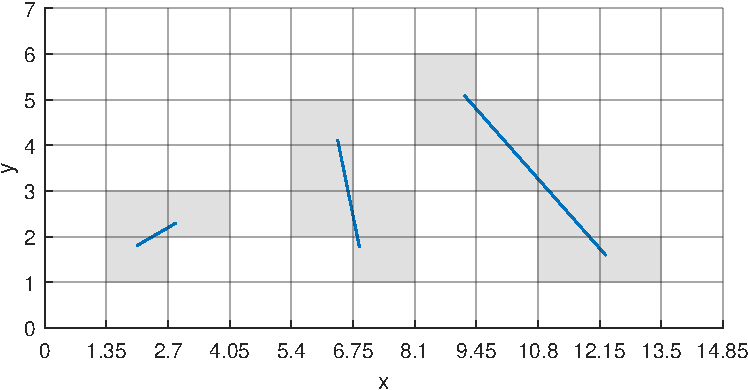
\includegraphics[width=.85\textwidth]{examples_1p35}%
\caption{Examples for $a=1.35$, $b=1$; $\len=1$, $\len=2.4$ and $\len=4.7$
}%
\label{fig: examples}%
\end{figure}%

An equivalent formulation of the problem is obtained allowing segments of length $\len$ \emph{or smaller}. The equivalence is clear from the fact that reducing the length cannot increase the number of visited tiles. Either of these formulations will be referred to as the \emph{direct} problem.

The \emph{inverse} problem is, given $\tiles \in \mathbb N$, to determine the infimum length of all segments that visit at least $\tiles$ tiles. For real-valued lengths this infimum is not a minimum, because given a segment that visits $\tiles$ tiles, its length can always be reduced by some non-zero amount without changing the number of visited tiles. This is a consequence of the interior of each tile being an open set.

The direct and inverse problems are closely related. Namely, if $\len$ is the infimum of all lengths that allow visiting at least $\tiles$ tiles (inverse problem), $\tiles$ is the maximum number of tiles that can be visited with lengths slightly greater than $\len$ (direct problem).

To address the remaining two questions, the notion of a \emph{random} segment of a given length needs to be precisely defined. This is done as follows. By symmetry, one endpoint of the segment can be assumed to lie in a fixed, reference tile. The position of this endpoint is \emph{uniformly} distributed on the tile. The segment orientation has a \emph{uniform} distribution on the set of all possible directions, and is \emph{independent} of the endpoint position. Solving the problem of how many tiles the segment visits on average, as will be seen, also answers the inverse question (segment length to visit a given number of tiles on average). A natural, related question is with what probability the segment visits the maximum number of tiles. 

% ***Do we need to discuss potential applications of this (if we can find any)? This probably depends on the journal
% ***Do we need a section with conclusions? Probably not; depends on the journal

The problems studied in this paper are related to Buffon's needle problem and Laplace's extension of it. Buffon's original problem considers tossing a needle of length $\len$ onto ruled paper with parallel lines a distance $b$ apart, and asks what is the probability of the needle crossing a line if it lands in a uniformly random position and orientation. For a needle of length $\len = b$, this is $2/\pi$, and hence repeated trials of this experiment can be used to estimate $\pi$. This is generalized in \cite{Ramaley69} to $2\len /(\pi b)$ for the expected number of crossings of a needle with arbitrary length.

The Buffon-Laplace needle problem \cite{Mathai99} considers a needle tossed onto a grid of rectangular tiles of width $a$ and height $b$. The number of visited tiles equals one plus the number of crossings almost surely. The probability of the needle staying within a single rectangle, that is visiting only one tile, is computed in \cite{Arnow94} for the case where $\len < \min(a,b)$. One of the results in this paper, as has been mentioned, is the complementary question of the probability that the needle visits the maximum number of tiles possible for its length.

The rest of the paper is organized as follows. Fundamental results are presented in \S\ref{part: fund results}, which form the basis of the subsequent analysis. The direct and inverse problems for a deterministic segment are considered in \S\ref{part: max}, first for arbitrary grids and then for a square grid. The analysis for the random segment is carried out in \S\ref{part: rand}. The average number of tiles is computed for arbitrary grids, and the probability that the segment visits the maximum number of tiles is obtained for a square grid.

% The rounding down (floor) and rounding up (ceiling) operations will be denoted as $\lfloor \cdot \rfloor$ and $\lceil \cdot \rceil$. The notation $[\mathsf S]$ will be used for the Iverson function, which equals $1$ if statement $\mathsf S$ is true and $0$ otherwise.


\section{Fundamentals}
\label{part: fund results}

For a grid with horizontal spacing $a$ and vertical spacing $b$, lines of the form $x = ka$ or $y = kb$ with $k \in \mathbb Z$ will be called \emph{grid lines}. A \emph{tile} is delimited by two pairs of consecutive horizontal and vertical grid lines. The intersection points of horizontal and vertical grid lines will be called \emph{grid points}. These correspond to vertices of the tiles.

Every segment has an associated \emph{discrete bounding rectangle}, which is the minimum-size rectangle that is formed by grid lines and contains the segment. More specifically, if the segment has endpoints $(x_1,y_1)$, $(x_2,y_2)$, where $x_1, x_2, y_1, y_2 \in \mathbb R$, its discrete bounding rectangle has lower-left corner and upper-right corner given as
\begin{align*}
& (\lfloor\min\{x_1, x_2\}/a\rfloor a, \lfloor\min\{y_1,y_2\}/b\rfloor b), \\
& (\lceil\max\{x_1, x_2\}/a \rceil a, \lceil\max\{y_1,y_2\}/b \rceil b).
\end{align*}
The dimensions of the discrete bounding rectangle, normalized to the tile width and height respectively, are two integer numbers $i$, $j$. Two examples are illustrated in Figure~\ref{fig: discrete bounding rectangle and touched tiles}, both with $i=5$, $j=4$. Clearly, all tiles visited by the segment are contained in the discrete bounding rectangle. Note also that the rectangle can have $i=0$ or $j=0$ if the segment coincides with part of a grid line.

\begin{figure}
\centering%
\subfigure[The segment does not pass through any interior grid points]{%
\label{fig: S_nogridpoints}%
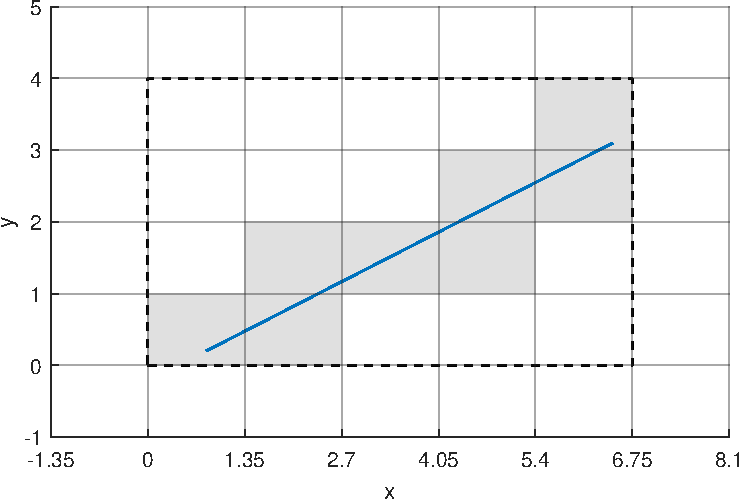
\includegraphics[width=.49\textwidth]{S_nogridpoints_1p35}%
}\hfill%
\subfigure[The segment passes through some interior grid points]{%
\label{fig: S_gridpoints}%
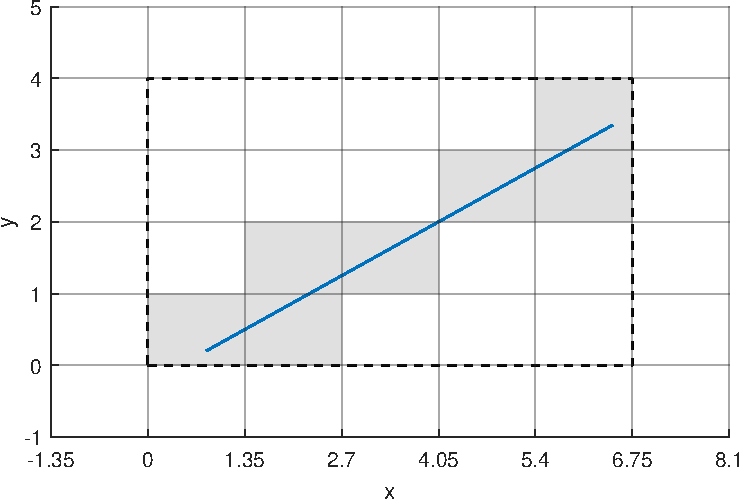
\includegraphics[width=.49\textwidth]{S_gridpoints_1p35}%
}%
\caption{Discrete bounding rectangle and visited tiles
}%
\label{fig: discrete bounding rectangle and touched tiles}%
\end{figure}%

\begin{proposition}
\label{prop: i+j-1}
Consider an arbitrary segment, and let $i, j$ respectively denote the normalized width and height of its discrete bounding rectangle. If $i, j \geq 1$, the number of tiles visited by the segment is at most $i+j-1$. This bound is attained if and only if the segment does not pass through any grid point in the interior of the rectangle.
\end{proposition}

\begin{proof}
The segment visits, by definition, two tiles in opposite corners of the discrete bounding rectangle. It can be assumed, without loss of generality, that those tiles are in the lower-left and upper-right corners of the rectangle, as in Figure~\ref{fig: discrete bounding rectangle and touched tiles}. The visited tiles can be thought of as following a path within the discrete bounding rectangle. Starting at the lower-left tile, the next tile can be the one to the left, the one above, or the one above and to the left. The latter case occurs if and only if the segment passes through the grid point between those two tiles.

Since the segment follows a straight line, once it ``leaves'' a row of tiles in its path from the lower-left to the upper-right corner, it can never visit any more tiles from that row. The same observation applies to the columns.

This implies that the maximum number of visited tiles is $i+j-1$, which is attained if and only if the segment avoids all grid points in the interior of the discrete bounding rectangle, as in Figure~\ref{fig: S_nogridpoints}. Note that grid points at the corners of the rectangle do not count for this; and that the segment cannot pass through any other grid points on the rectangle border, because that would imply $i=0$ or $j=0$. Figure~\ref{fig: S_gridpoints} illustrates a case where the maximum is not attained.
\end{proof}

\begin{proposition}
\label{prop: len ineq i j}
Consider $a, b, \len \in \mathbb R^+$ and $i, j \in \mathbb N$, $i, j \geq 2$ arbitrary.
\begin{enumerate}
\item
\label{prop: len ineq i j: ineqs}
The following inequalities hold for any segment with length $\len$ whose discrete bounding rectangle has normalized dimensions $i, j$:
\begin{align}
\label{eq: len > sqrt}
\len &> \sqrt{(i-2)^2 a^2 + (j-2)^2 b^2}, \\
\label{eq: len leq sqrt}
\len &\leq \sqrt{i^2 a^2 + j^2 b^2}.
\end{align}
\item
\label{prop: len ineq i j: exist}
Conversely, if $\len$, $i$, $j$ satisfy \eqref{eq: len > sqrt} and \eqref{eq: len leq sqrt} there exists a segment of length $\len$ whose discrete bounding rectangle has normalized dimensions $i$ and $j$.
\item
\label{prop: len ineq i j: ineq, exist}
There is a segment of length not exceeding $\len$ that has a discrete bounding rectangle with normalized dimensions $i, j$ if and only if \eqref{eq: len > sqrt} holds.
\end{enumerate}
\end{proposition}

\begin{proof}
\ref*{prop: len ineq i j: ineqs} The inequalities follow from the fact that the segment endpoints lie in the interiors or on the outer edges of two tiles in opposite corners of the discrete bounding rectangle. This is illustrated in Figures~\ref{fig: len ineq 4 3} and \ref{fig: len ineq 4 2} for two specific $(i,j)$ pairs respectively. For each $(i,j)$, segments are shown with lengths close to either of the two bounds. Note that \eqref{eq: len > sqrt} is valid even for $i=2$, $j=2$, in which case it reduces to $\len>0$.

\ref*{prop: len ineq i j: exist} For $a$, $b$, $\len$, $i$, $j$ satisfying the two inequalities, a segment of length $\len$ can be found that has its endpoints in the interiors or on the outer edges of the two shaded tiles of a rectangle of normalized dimensions $i$ and $j$, as in Figure~\ref{fig: len ineq i j}, which is thus the discrete bounding rectangle of that segment.
\begin{figure}
\centering%
\subfigure[$i=4$, $j=3$]{%
\label{fig: len ineq 4 3}%
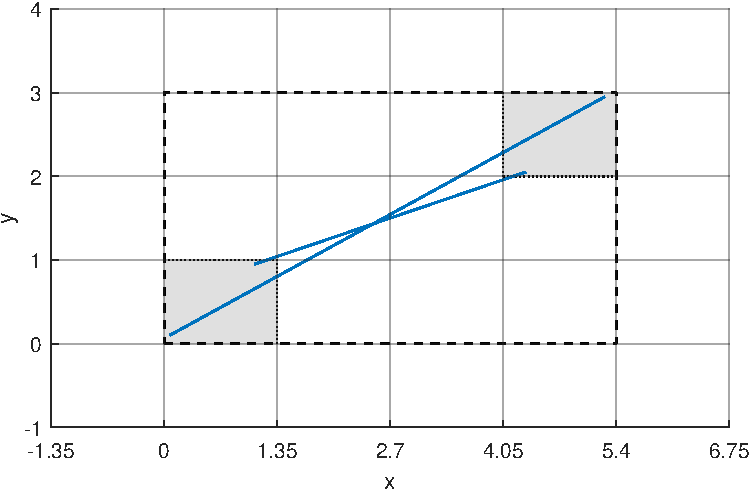
\includegraphics[width=.49\textwidth]{L_ineq_4_3_1p35}%
}\hfill%
\subfigure[$i=4$, $j=2$]{%
\label{fig: len ineq 4 2}%
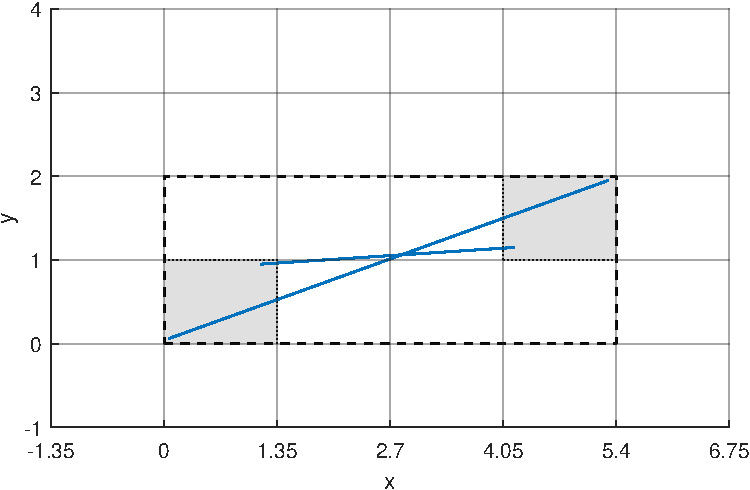
\includegraphics[width=.49\textwidth]{L_ineq_4_2_1p35}%
}%
\caption{Relationship between segment length $\len$ and dimensions $i$, $j$ of the discrete bounding rectangle
}%
\label{fig: len ineq i j}
\end{figure}%

\ref*{prop: len ineq i j: ineq, exist} ``\eqref{eq: len > sqrt} $\Rightarrow$ there is a segment\ldots'': Assume that \eqref{eq: len > sqrt} holds. It is always possible to choose a length equal to or smaller than $\len$ such that both \eqref{eq: len > sqrt} and \eqref{eq: len leq sqrt} hold. The result follows, for that length, from part~\ref{prop: len ineq i j: exist}.

``There is a segment\ldots $\Rightarrow$ \eqref{eq: len > sqrt} '': Assume that a segment exists with length not exceeding $\len$ and with a discrete bounding rectangle with normalized dimensions $i$, $j$. From part~\ref{prop: len ineq i j: ineqs}, inequality \eqref{eq: len > sqrt} holds for that segment length, and thus for $\len$.
\end{proof}

According to Proposition~\ref{prop: i+j-1}, in order to maximize the number of visited tiles for a given length, the position and orientation of the segment should be chosen to obtain $i+j-1$ as large as possible, where $i$ and $j$ are the normalized dimensions of its discrete bounding rectangle. On the other hand, Proposition~\ref{prop: len ineq i j} restricts the $i, j$ values that can be achieved with a given length. A relevant question is: are there any $(i,j)$ pairs that can be disregarded irrespective of the length $\len$? In other words, what is the ``smallest'' subset of $\mathbb N^2$ such that the $(i,j)$ pair that maximizes the number of tiles for any given length can always be found within that subset?

For instance, it is clear from Figure~\ref{fig: examples} that segment orientations near the vertical or horizontal directions (resulting in $i=1$ with large $j$, or $j=1$ with large $i$) will not maximize the number of visited tiles, and thus the corresponding $(i,j)$ pairs can be discarded. On the other hand, the set of optimal $(i,j)$ pairs must contain one such pair for each possible value of $i+j-1$, so that the set can produce that value as the solution (maximum number of visited tiles) for certain lengths. It is insightful to examine two specific examples before giving an explicit formula for the coordinates of the optimal pairs.

Consider $a=b=1$ first. This is illustrated in Figure~\ref{fig: ijLS_1}. Note that in this and in the next figures the axes represent $ia$ and $jb$, rather than
% normalized coordinates
$i$ and $j$. In this graph, each dashed diagonal line contains pairs $(ia,jb)$ with the same $i+j-1$; and the lower bound \eqref{eq: len > sqrt} corresponds to an arc centered at $(2a,2b)$.

\begin{figure}
\centering%
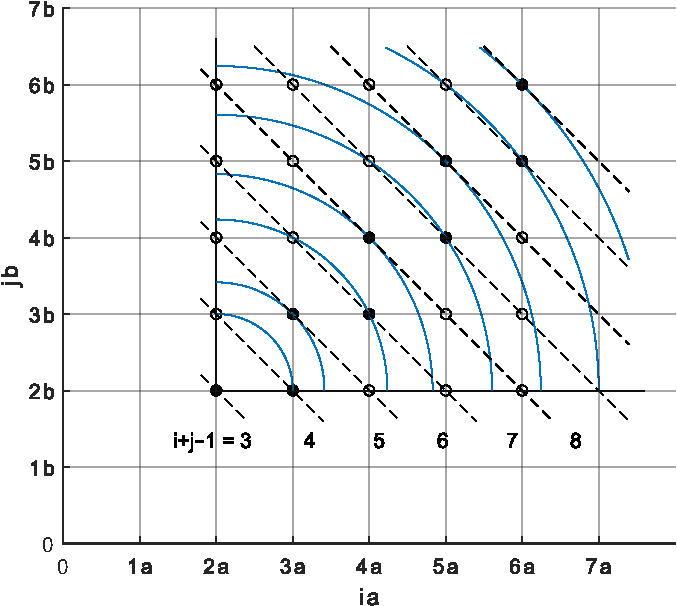
\includegraphics[width=.7\textwidth]{ijLS_1}%
\caption{Relationship of segment length and number of visited tiles with the width and height of the discrete bounding rectangle, for $a=b$
}%
\label{fig: ijLS_1}%
\end{figure}%
% ***Maybe combine this figure and the next into one figure with two subfigures (stacked vertically, size similar to now). Not sure. It has been done in others

For a given $\len \in \mathbb R^+$, the $(i,j)$ pairs that can be achieved with segments of length not exceeding $\len$ are, by Proposition~\ref{prop: len ineq i j}.\ref{prop: len ineq i j: ineq, exist}, those that satisfy \eqref{eq: len > sqrt}. Thus for a given value of $i+j-1$ the optimal $(i,j)$ pair (the one that can be achieved with the smallest possible length) is determined by the condition that the point $(ia,jb)$ minimizes the distance to $(2a,2b)$. Such pairs are depicted as filled circles in the figure. The displayed arcs represent the inequality \eqref{eq: len > sqrt} for each of the optimal pairs. Conversely, given a length $\len$, the maximum number of visited tiles will be achieved with one of these pairs, namely the pair $(i,j)$ such that $(ia,jb)$ is on the highest (or rightmost) diagonal line while still being contained in the circle of radius $\len$ centered at $(2a,2b)$.

The optimal pairs in this specific case have $j=i$ or $j=i-1$, as seen in the figure. Due to symmetry, any pair $(i,i-1)$ could be replaced by $(i-1,i)$. This illustrates that the set of optimal pairs is not unique in general. 

As a second example, consider $a=1.35$, $b=1$. This is depicted in Figure~\ref{fig: ijLS_1p35}. Again, the optimal pair $(i,j)$ for each diagonal is that for which the point $(ia,jb)$ is closest to $(2a,2b)$; but in this case the $i$, $j$ coordinates of these pairs do not follow a rule as simple as in the previous example.

\begin{figure}
\centering%
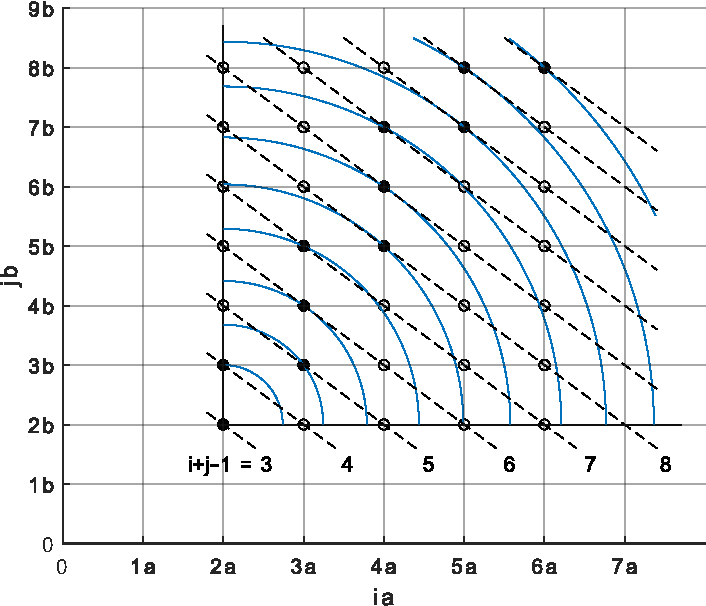
\includegraphics[width=.7\textwidth]{ijLS_1p35}%
\caption{Relationship of segment length and number of visited tiles with the width and height of the discrete bounding rectangle, for $a=1.35b$
}%
\label{fig: ijLS_1p35}%
\end{figure}%

The following proposition gives an explicit method to obtain a set of optimal $(i,j)$ pairs. This set will be denoted as $\mss = \{(i_3,j_3), (i_4.j_4), \ldots\}$, where the pair $(i_\tiles,j_\tiles)$ corresponds to $i+j-1 = \tiles$.

\begin{proposition}
\label{prop: min suff set, form}
Given $a, b \in \mathbb R^+$ and $\tiles \in \mathbb N$, $\tiles \geq 3$, a set of optimal pairs $\mss = \{(i_3,j_3), (i_4.j_4), \ldots\}$ can be obtained as
\begin{align}
\label{eq: min suff set, form, i}
i_\tiles &= \left\lfloor \frac{(\tiles-3) b^2}{a^2+b^2} + \frac 5 2 \right\rfloor, \\
\label{eq: min suff set, form, j}
j_\tiles &= \left\lceil  \frac{(\tiles-3) a^2}{a^2+b^2} + \frac 3 2 \right\rceil,
\end{align}
where $i_\tiles + j_\tiles-1 = \tiles$. All pairs $(i_\tiles,j_\tiles)$ are strictly below the line
\begin{equation}
\label{eq: upper bound, line}
j = \frac{i a^2}{b^2} - \frac{3a^2}{2b^2} + \frac 5 2,
\end{equation}
and above or on the line
\begin{equation}
\label{eq: lower bound, line}
j = \frac{i a^2}{b^2} - \frac{5a^2}{2b^2} + \frac 3 2.
\end{equation}
\end{proposition}

\begin{proof}
For each $\tiles$, the pair $(i_\tiles,j_\tiles)$ should be chosen as that on the line $i+j-1=\tiles$ which minimizes $(i-2)^2 a^2 + (j-2)^2 b^2$. This allows maximizing the sum $i+j-1$, and thus the number of visited tiles, for a given length restriction (direct problem); or minimizing the required lengths for a specified number of visited files (inverse problem).

Consider, for the moment, $i$, $j$ as if they were real-valued variables, and denote $x=ia$, $y=jb$. The line $i+j-1 = \tiles$ then becomes
\begin{equation}
\label{eq: line 1}
\frac x a + \frac y b = \tiles + 1,
\end{equation}
and $(i-2)^2 a^2 + (j-2)^2 b^2$ is expressed as $(x-2a)^2+(y-2b)^2$. The point minimizing this quadratic function along \eqref{eq: line 1} is the intersection of that line with the perpendicular line passing through $(2a,2b)$, that is,
\begin{equation}
\label{eq: line 2}
y = \frac {a (x-2a)} b + 2b.
\end{equation}
This is depicted for $a=1.35$, $b=1$, $\tiles=7$ in Figure~\ref{fig: min suff set, form}, where \eqref{eq: line 2} is shown with solid line. Solving the system of equations \eqref{eq: line 1} and \eqref{eq: line 2} gives 
\begin{align}
\frac x a - 2 &= \frac{(t-3)b^2}{a^2+b^2}, \\
\frac y b - 2 &= \frac{(t-3)a^2}{a^2+b^2}.
\end{align}
In terms of the real-valued variables $i$, $j$, the solution $(\isolr, \jsolr)$ is
\begin{align}
\label{eq: prop: min suff set, form: isolr}
\isolr &= \frac{(t-3)b^2}{a^2+b^2} + 2, \\
\label{eq: prop: min suff set, form: jsolr}
\jsolr &= \frac{(t-3)a^2}{a^2+b^2} + 2.
\end{align}
The corresponding point $(\isolr a, \jsolr b)$ is shown in Figure~\ref{fig: min suff set, form} with a square marker.

\begin{figure}%
\centering%
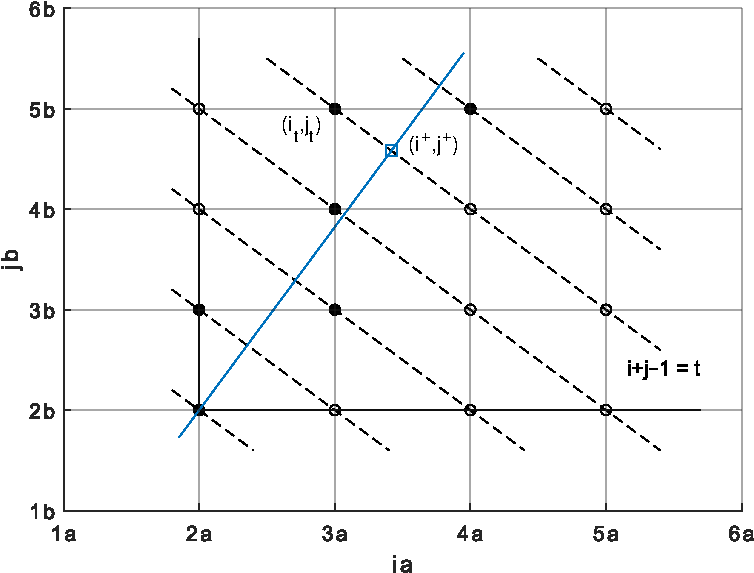
\includegraphics[width=.7\textwidth]{mss}%
\caption{Obtaining $(\isolr, \jsolr)$ and $(i_\tiles, j_\tiles)$ in  Proposition~\ref{prop: min suff set, form}. Example with $a=1.35$, $b=1$, $\tiles=7$%
}%
\label{fig: min suff set, form}%
\end{figure}%

The variables $i$, $j$ are actually limited to integer values. The pair $(i_\tiles, j_\tiles)$ that minimizes $(i-2)^2 a^2 + (j-2)^2 b^2$ along the line $i+j-1=\tiles$ restricted to integer values is either $(\lceil \isolr \rceil, \lfloor \jsolr \rfloor)$ or $(\lfloor \isolr \rfloor, \lceil \jsolr \rceil)$, whichever gives $(i_\tiles a, j_\tiles b)$ closest to $(\isolr a, \jsolr b)$, as illustrated in Figure~\ref{fig: min suff set, form}. In case of a tie the first of the two pairs is chosen. This can be expressed as
\begin{align}
\label{eq: prop: min suff set, form: isoli}
i_\tiles &= \left\lfloor \isolr + \frac 1 2 \right\rfloor, \\
\label{eq: prop: min suff set, form: jsoli}
j_\tiles &= \left\lceil \jsolr - \frac 1 2 \right\rceil,
\end{align}
which corresponds to rounding $\isolr$ and $\jsolr$ to the closest integers, with ties resolved in opposite directions. Combining \eqref{eq: prop: min suff set, form: isolr}--\eqref{eq: prop: min suff set, form: jsoli}
% *!*
yields \eqref{eq: min suff set, form, i} and \eqref{eq: min suff set, form, j}.

From \eqref{eq: prop: min suff set, form: isolr} and \eqref{eq: prop: min suff set, form: isoli},
\begin{equation}
\label{eq: prop: min suff set, form: isoli ineq}
\frac{(t-3)b^2}{a^2+b^2} + \frac 3 2 < i_\tiles \leq \frac{(t-3)b^2}{a^2+b^2} + \frac 5 2,
\end{equation}
and similarly, from \eqref{eq: prop: min suff set, form: jsolr} and \eqref{eq: prop: min suff set, form: jsoli},
\begin{equation}
\label{eq: prop: min suff set, form: jsoli ineq}
\frac{(t-3)a^2}{a^2+b^2} + \frac 3 2 \leq j_\tiles < \frac{(t-3)a^2}{a^2+b^2} + \frac 5 2.
\end{equation}
Considering the first inequality in \eqref{eq: prop: min suff set, form: isoli ineq} and the second in \eqref{eq: prop: min suff set, form: jsoli ineq} as equalities and eliminating $\tiles$ gives \eqref{eq: upper bound, line}. The pair $(i_\tiles, j_\tiles)$ is strictly below the line \eqref{eq: upper bound, line} because the used inequalities are strict. Similarly, the bounding line \eqref{eq: lower bound, line} results from the second inequality in \eqref{eq: prop: min suff set, form: isoli ineq} and the first in \eqref{eq: prop: min suff set, form: jsoli ineq}, and the fact that both inequalities are not strict implies that the bound \eqref{eq: lower bound, line} can actually be attained.
\end{proof}

The bounding lines in Proposition~\ref{prop: min suff set, form} are shown in Figure~\ref{fig: pairs_bounds}, using three different pairs of grid parameters $a$, $b$ as examples. Given $(i_\tiles,j_\tiles) \in \mss$, the next pair $(i_{\tiles+1},j_{\tiles+1})$ is obtained by incrementing $j$ if that results in a point below \eqref{eq: upper bound, line}. Else $i$ is incremented instead, and the new pair is guaranteed to be above or on \eqref{eq: lower bound, line}.

\begin{figure}
\centering%
\subfigure[$a = 1$, $b = 1$]{%
\label{fig: pairs_bounds_1}%
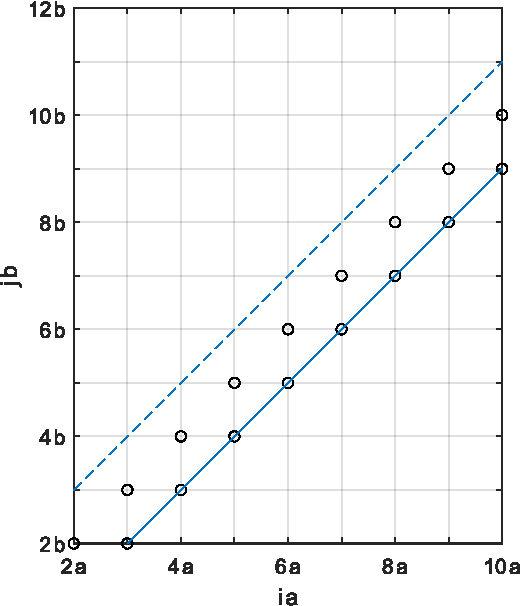
\includegraphics[height=.24\textheight]{pairs_bounds_1}% *!*
}\hfill%
\subfigure[$a = 1.35$, $b = 1$]{%
\label{fig: pairs_bounds_1p35}%
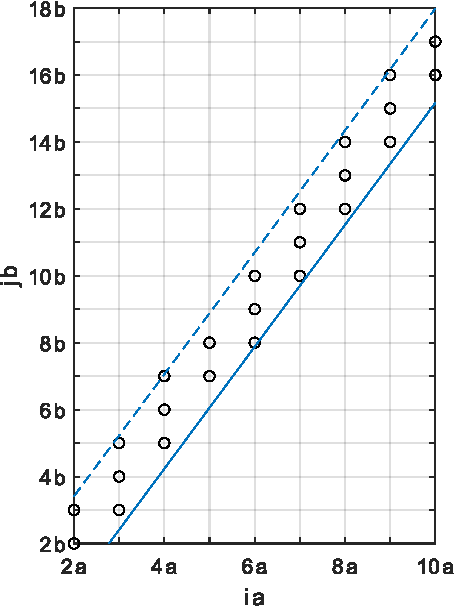
\includegraphics[height=.24\textheight]{pairs_bounds_1p35}% *!*
}\hfill%
\subfigure[$a = \sqrt{2}$, $b = 1$]{%
\label{fig: pairs_bounds_sqrt2}%
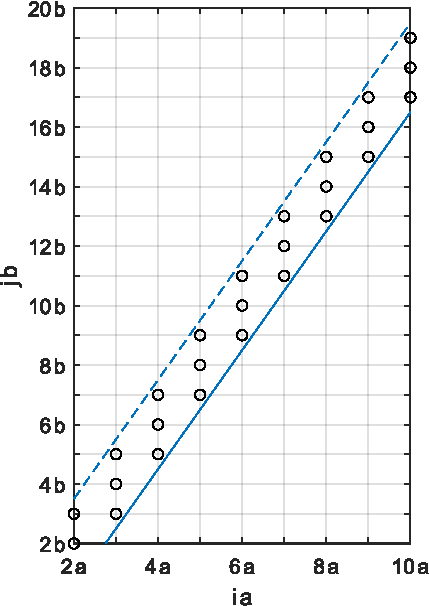
\includegraphics[height=.24\textheight]{pairs_bounds_sqrt2}% *!*
}%
\caption{Set of optimal pairs $\mss$, and bounding lines
}%
\label{fig: pairs_bounds}%
\end{figure}%
 
For $a^2/b^2$ arbitrary, the number of pairs in $\mss$ with the same $i$ coordinate, or with the same $j$, is in general irregular, because the lines \eqref{eq: upper bound, line} and \eqref{eq: lower bound, line} do not follow a ``natural'' direction of the grid. This happens for instance in Figure~\ref{fig: pairs_bounds_1p35}, where the number of pairs for each $i$ equals either $2$ or $3$ without a clear pattern.\footnote{Strictly, there is a periodic pattern whenever $a^2/b^2$ is rational, which is the case in Figure~\ref{fig: pairs_bounds_1p35}. However, it is not easily discernible unless $a^2/b^2$ is a ratio of small numbers.}
On the other hand, a simple pattern arises when $a^2/b^2$ or $b^2/a^2$ is a natural number, as seen in Figures~\ref{fig: pairs_bounds_1} and \ref{fig: pairs_bounds_sqrt2}.

A segment whose discrete bounding rectangle has normalized width $i$ and height $j$ is oriented with approximate slope $jb/(ia)$ with respect to the $x$ axis (see Figure~\ref{fig: len ineq i j}); and this approximation becomes better for greater segment lengths. From \eqref{eq: upper bound, line} and \eqref{eq: lower bound, line} it can be seen that the positions of the pairs $(i,j) \in \mss$ have $j/i \approx a^2/b^2$ for large $i, j$. Therefore the optimal slope for long segments is approximately $a/b$. This formalizes the intuition that to maximize the number of visited tiles, the segment should follow a direction along which the perceived ``length'' of the tile is smaller.
% but not ``smallest'', if that were the case it would always be either vertical or horizontal


\section{Direct and inverse problems for a deterministic segment}
\label{part: max}

The direct and inverse problems defined in \S\ref{part: intro}, considering the segment position and orientation as deterministic, are addressed in this section. The general case for rectangular grids with real-valued segment lengths is analyzed first, in \S\ref{part: max: arbitrary grid, real lengths}. The particular case of square grids is addressed in \S\ref{part: max: unit square grid, real lengths}, as it allows a specialized formula for the direct problem. Lastly, the analysis of a unit square grid with integer-valued lengths is presented in \S\ref{part: max: unit square grid, integer lengths}.


\subsection{Arbitrary grid with real-valued lengths}
\label{part: max: arbitrary grid, real lengths}

For a grid with parameters $a, b \in \mathbb R^+$, the maximum number $\tiles$ of visited tiles with a given real-valued length $\len$ can be represented by a function $\funt: \mathbb R^+ \to \mathbb N$ such that $\tiles = \funt(\len)$. Similarly, for the inverse problem a function $\funl: \mathbb N \to \mathbb R^+$ can be defined such that $\funl(\tiles)$ gives the infimum length of all segments that visit at least $\tiles$ tiles.

The function $\funt$ can be obtained from $\funl$ by noting that the maximum number of tiles that can be visited by a segment of length $\len$ is the index of the largest term of the sequence $\funl(\tiles)$ that is less than $\len$:
\begin{equation}
\label{eq: funt funl}
\funt(\len) = \max \{\tiles \in \mathbb N \st \funl(\tiles)<\len\}.
\end{equation}
Conversely, $\funl$ can be obtained from $\funt$ as
\begin{equation}
\label{eq: funl funt}
\funl(\tiles) = \inf\{\len \in \mathbb R^+ \st \funt(\len) \geq \tiles\}.
\end{equation}

For arbitrary $a, b \in \mathbb R^+$, the functions $\funt$ and $\funl$ can be computed using an iterative procedure, which exploits the fact that the pairs $(i_3,j_3), (i_4,j_4), \ldots$ of $\mss$ are sorted by increasing $i+j-1$, and also by increasing $(i-2)^2 a^2 + (j-2)^2 b^2$. Namely, for $\funt$ the following procedure yields the solution: generate successive pairs to find the last one, $(i_\tiles,j_\tiles)$, that satisfies \eqref{eq: len > sqrt}; then $\funt(\len) = \tiles$. For $\funl$ the analogous method gives a direct formula. In addition, it is possible to obtain a direct formula also for $\funt$ using a different approach. These formulas are given in Theorems \ref{theo: funt, form} and \ref{theo: funl, form}.

\begin{theorem}
\label{theo: funt, form}
For $a, b \in \mathbb R^+$, $a \geq b$ and $\len \in \mathbb R^+$,
\begin{equation}
\label{eq: theo: funt, form; funt}
\funt(\len) = \isoli+\jsoli-1
\end{equation}
with
\begin{align}
\label{eq: theo: funt, form; i}
\isoli &= \left\lceil \frac{a + b \Re \sqrt{4\len^2/(a^2+b^2)-1}}{2a} \right\rceil + 1, \\
\label{eq: theo: funt, form; j}
\jsoli &= \left\lceil \frac{\sqrt{\len^2-(\isoli-2)^2a^2}}{b} \right\rceil + 1.
\end{align}
The function $\funt$ is piecewise constant and left-continuous, with unit-height jumps. A jump occurs at $\len$ if and only if $\len = \funl(\tiles)$ for some $\tiles \in \mathbb N$, $\tiles \geq 4$; and then $\funt(\len) = \tiles-1$, $\lim_{h \rightarrow 0+} \funt(\len+h) = \tiles$.
\end{theorem}

\begin{proof}
The approach is similar to that used in Proposition~\ref{prop: min suff set, form}. Namely, for $i, j \geq 2$ the intersection $(\isolr a, \jsolr b)$ of the line defined by \eqref{eq: lower bound, line} and the arc centered at $(2a,2b)$ with radius $\len$ is found, and from that the actual integer solution $(\isoli, \jsoli)$ is computed.

More specifically, assuming that \eqref{eq: lower bound, line} holds, the largest $i$ that can be achieved with lengths not exceeding $\len$ is obtained, as given by Proposition~\ref{prop: len ineq i j}.\ref{prop: len ineq i j: ineq, exist}. This value, $\isoli$, is computed by rounding down $\isolr$. Then, assuming that $i = \isoli$, the largest $j$ allowed by Proposition~\ref{prop: len ineq i j}.\ref{prop: len ineq i j: ineq, exist}, $\jsoli$, is obtained. As will be seen, in some cases the resulting $(\isoli,\jsoli)$ is in $\mss$ as defined by Proposition~\ref{prop: min suff set, form}, and in other cases it is not. However, in either case $(\isoli,\jsoli)$ has the largest $i+j-1$ sum that can be achieved with segments of length up to $\len$. Thus the desired result is $\isoli+\jsoli-1$.

The two possibilities are illustrated in Figure~\ref{fig: ijLS_1p35_detail} for $a=1.35$, $b=1$. In each case, the arc displayed in the graph is centered at $(2a,2b)$ and has radius $\len$. The inner region defined by the arc contains all $(ia,jb)$ points such that the pair $(i,j)$ is achievable according to Proposition~\ref{prop: len ineq i j}.\ref{prop: len ineq i j: ineq, exist}. As in previous figures, filled circles represent points $(ia,jb)$ such that $(i,j) \in \mss$. The solid line is the bound \eqref{eq: lower bound, line}. The intersection point $(\isolr a, \jsolr b)$ is displayed with a square marker.

\begin{figure}
\centering%
\subfigure[$\len = 3.1$: $(\isoli,\jsoli) \in \mss$]{%
\label{fig: ijLS_1p35_detail_in}%
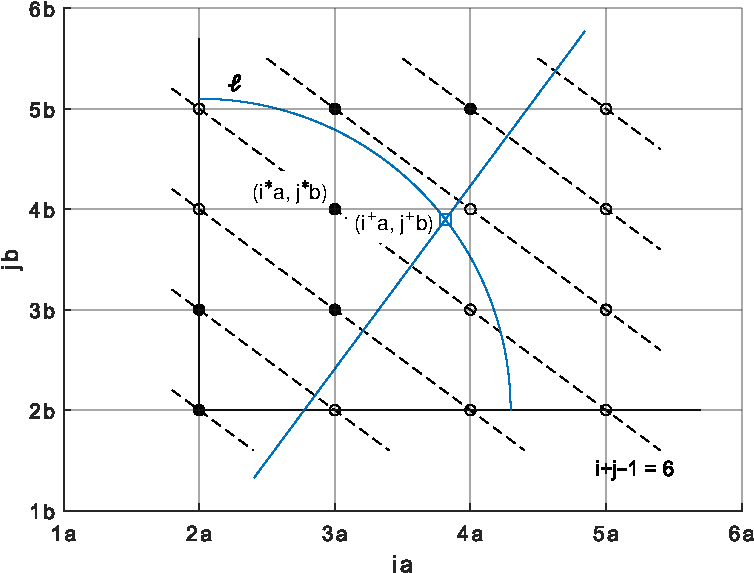
\includegraphics[width=.7\textwidth]{ijLS_1p35_detail_in}%
}\\%\hfill%
\subfigure[$\len = 3.7$: $(\isoli,\jsoli) \notin \mss$]{%
\label{fig: ijLS_1p35_detail_notin}%
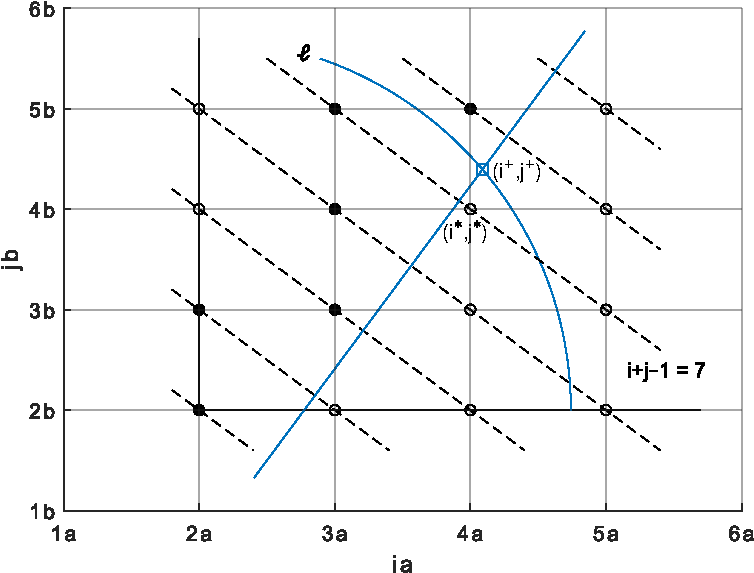
\includegraphics[width=.7\textwidth]{ijLS_1p35_detail_notin}%
}%
\caption{Obtaining $(\isoli,\jsoli)$ in Theorem~\ref{theo: funt, form}. Examples with $a=1.35$, $b=1$%
}%
\label{fig: ijLS_1p35_detail}%
\end{figure}%

The pair $(\isolr, \jsolr)$ can be obtained as a solution of the equation system
\begin{align}
\label{eq: icont jcont 1}
(\isolr-2)^2 a^2 + (\jsolr-2)^2 b^2 &= \len^2, \\
\label{eq: icont jcont 2}
\jsolr = \frac{\isolr a^2}{b^2} - \frac{5a^2}{2b^2} + \frac 3 2.
\end{align}
Substituting \eqref{eq: icont jcont 2} into \eqref{eq: icont jcont 1} yields a quadratic equation for $\isolr$,
\begin{equation}
\label{eq: quadratic, i}
4a^2(\isolr-2)^2 - 4a^2(\isolr-2) + a^2+b^2-\frac{4\len^2 b^2}{a^2+b^2},
\end{equation}
which can have zero, one or two real-valued solutions (this respectively means that the line \eqref{eq: icont jcont 2} is exterior, tangent or secant to the circle \eqref{eq: icont jcont 1}). Only the solution with $\isolr, \jsolr \geq 2$, if any, is of interest. This solution can only exist as the one with largest $\isolr$ value when there are real-valued solutions, and it is obtained as
\begin{equation}
\label{eq: icont jcont 3}
\isolr = \frac{a + b \sqrt{4\len^2/(a^2+b^2)-1}}{2a} + 2.
\end{equation}

The case with no real-valued solutions to \eqref{eq: quadratic, i} corresponds to $\len < \sqrt{a^2+b^2}/2$. Since $a \geq b$, this implies that $\len < a$. Thus any achievable $(i,j)$ pair, if any, will have $i=2$. Therefore in this case $\isoli$ should be set to $2$; and then the maximum achievable $\jsoli$ will be obtained from \eqref{eq: icont jcont 2}.

If \eqref{eq: quadratic, i} has two real-valued solutions or one real-valued double solution, which is the case when $\len \geq \sqrt{a^2+b^2}/2$, the largest solution will have $\jsolr < 2$ if $\isolr < (b^2/a^2+5)/2$, as can be seen setting $\jsolr=2$ in \eqref{eq: icont jcont 2}; or equivalently if $\sqrt{a^2+b^2}/2 \leq \len < (a^2+b^2) / (2a)$, as can be seen substituting $\jsolr < 2$ and $\isolr < (b^2/a^2+5)/2$ in \eqref{eq: icont jcont 1}. Since $\isolr < (b^2/a^2+5)/2 < 3$ for $a \geq b$, only pairs with $i=2$ are achievable in this case again, and thus the solution $\isoli$ should also be $2$.

Lastly, for $\len \geq (a^2+b^2) / (2a)$ the expressions \eqref{eq: icont jcont 2} and \eqref{eq: icont jcont 3} give $\isolr, \jsolr \geq 2$, and $\isoli$ should be taken as the greatest integer less than $\isolr$, i.e.~$\lceil \isolr \rceil-1$.
 
The three cases are unified by taking the real part of \eqref{eq: icont jcont 3} and computing $\isoli = \lceil \isolr \rceil-1$, as is easily checked. This gives \eqref{eq: theo: funt, form; i}. Once $\isoli$ is known, $\jsoli$ is computed, according to \eqref{eq: theo: funt, form; j}, as the greatest integer such that $(\isoli a,\jsoli b)$ is within the circle determined by $\len$. This ensures that $(\isoli,\jsoli)$ is achievable with lengths less than $\len$.

There are two possibilities for the pair $(\isoli,\jsoli)$, as stated at the outset. These are illustrated in Figures~\ref{fig: ijLS_1p35_detail_in} and \ref{fig: ijLS_1p35_detail_notin} respectively. The first possibility is that $(\isoli,\jsoli) \in \mss$ (Figure~\ref{fig: ijLS_1p35_detail_in}). Then, by construction  $(\isoli,\jsoli)$ maximizes $i+j-1$ among all achievable pairs of $\mss$, and is therefore optimal.

The second possibility is that $(\isoli,\jsoli) \notin \mss$ (Figure~\ref{fig: ijLS_1p35_detail_notin}). This happens when the pair from $\mss$ that has $i = \isoli$ ($(4,5)$ in the figure) is outside the circle, i.e.~it would require a length greater than $\len$. The selected $(\isoli,\jsoli)$ ($(4,4)$ in the figure), however, has the same $i+j-1$ sum as the pair from $\mss$ that ``should'' be used, which is $(\isoli-1,\jsoli+1)$ ($(3,5)$ in the figure); and therefore gives the same result. This is always the case, because  $(\isoli,\jsoli+1) \in \mss$ (it is above or on the bounding line) and $(\isoli,\jsoli) \notin \mss$ (it is below the line), and due to how $\mss$ has been constructed, this implies that $(\isoli-1,\jsoli+1) \in \mss$ and $(\isoli-1,\jsoli+k) \notin \mss$ for $k =2, 3, \ldots$.  Therefore, $(\isoli,\jsoli)$ is achievable and maximizes $i+j-1$, which implies that $\isoli+\jsoli-1$ is the desired solution.

Therefore, regardless of whether $(\isoli,\jsoli)$ is in $\mss$ or not, \eqref{eq: theo: funt, form; i} and \eqref{eq: theo: funt, form; j} give $\isoli+\jsoli-1$ equal to $\funt(\len)$, as claimed.

It should be noted that for the specific case that $a^2/b^2 = 2k-1$, $k \in \mathbb N$ the lower bounding line \eqref{eq: lower bound, line} becomes $j = i(2k-1)-5k+4$, which gives integer $j$ for integer $i$. This means that the bound is actually achieved for all pairs in $\mss$ (see for example Figure~\ref{fig: pairs_bounds_1}), and the case $(\isoli,\jsoli) \notin \mss$ never occurs. Thus, when $a^2/b^2$ is an odd integer the obtained $(\isoli,\jsoli)$ is guaranteed to be in $\mss$, whereas for general $a^2/b^2$ either $(\isoli,\jsoli)$ or $(\isoli-1,\jsoli+1)$ are in in this set.
% ^ If this is needed outside of the proof, it can be included at the end of the theorem statement

As for the properties of $\funt$, it follows from \eqref{eq: theo: funt, form; funt}--\eqref{eq: theo: funt, form; j} that this function is piecewise constant and left-continuous. From the procedure described in the previous paragraphs for obtaining $(\isoli, \jsoli)$ it is clear that $\isoli+\jsoli-1$ increases in steps of $1$ when $\len$ is increased continuously; that is, $\funt$ has jumps of unit height.

Consider an arbitrary $\len$ such that for some $\tiles \in \mathbb N$, $\tiles \geq 4$
\begin{equation}
\label{eq: theo funt, form: prop 1}
\funl(\tiles)=\len.
\end{equation}
To see that $\funt$ has a jump at $\len$, assume for the sake of contradiction that $\funt$ is continuous, therefore constant, at that point. Then there is $\epsilon > 0$ for which $\funt(\len+\epsilon) = \tiles = \funt(\len-\epsilon)$. This means that there exists a segment with length $\len-\epsilon$ that visits $\tiles$ tiles, and thus $\funl(\tiles) \leq \len-\epsilon < \len$, in contradiction with \eqref{eq: theo funt, form: prop 1}. Therefore $\funt$ is discontinuous, from the right, at $\len$. By definition of $\funl$, \eqref{eq: theo funt, form: prop 1} implies that $\funt(\len) < \tiles$, and that there exists $\epsilon > 0$ such that $\funt(\len+h) = \tiles$ for $0 < h < \epsilon$. This means that
\begin{align}
\label{eq: theo funt, form: prop 2}
\funt(\len) &< \tiles, \\
\label{eq: theo funt, form: prop 3}
\lim_{h \rightarrow 0+} \funt(\len+h) &= \tiles,
\end{align}
that is, $\funt$ has a jump at $\len$. In addition, since the jump has unit height, it follows from \eqref{eq: theo funt, form: prop 2} and \eqref{eq: theo funt, form: prop 3}  that $\funt(\len) = \tiles-1$.

Conversely, assume that \eqref{eq: theo funt, form: prop 2} and \eqref{eq: theo funt, form: prop 3} hold for some $\len \in \mathbb R^+$, $\tiles \in \mathbb N$. From \eqref{eq: theo funt, form: prop 2} it follows that  $\funl(\tiles) \geq \len$. On the other hand, \eqref{eq: theo funt, form: prop 3} implies that $\funl(\tiles) \leq \len$. Thus $\funl(\tiles)=\len$.
\end{proof}

Although Theorem~\ref{theo: funt, form} is valid for $a \geq b$, the result could be applied for $a < b$ by simply swapping the values of $a$ and $b$. In other words, \eqref{eq: theo: funt, form; funt}--\eqref{eq: theo: funt, form; j}
% *!*
can be used for any grid if $a$, $b$ are interpreted as the largest and smallest sides of a tile, respectively.

\begin{theorem}
\label{theo: funl, form}
For $a, b \in \mathbb R^+$ and $\tiles \in \mathbb N$,
\begin{equation}
\label{eq: theo: funl, form; funl}
\funl(\tiles) = \sqrt{(\isoli-2)^2 a^2 + (\jsoli-2)^2 b^2}
\end{equation}
with
\begin{align}
\label{eq: theo: funl, form; isolr}
\isolr &= \max\left\{ \frac{(\tiles-3) b^2}{a^2+b^2}, 0 \right\} + 2, \\
\label{eq: theo: funl, form; jsolr}
\jsolr &= \max\left\{ \frac{(\tiles-3) a^2}{a^2+b^2}, 0 \right\} + 2, \\
\label{eq: theo: funl, form; isoli}
\isoli &= \left\lfloor \isolr + \frac 1 2 \right\rfloor, \\
\label{eq: theo: funl, form; jsoli}
\jsoli &= \left\lceil \jsolr - \frac 1 2 \right\rceil.
\end{align}
Equivalently, for $\tiles \geq 3$,
\begin{equation}
\label{eq: theo: funl, form; funl 2}
\funl(\tiles) = \sqrt{\frac{(t-3)^2 a^2 b^2}{a^2+b^2} + \roundterm^2(a^2+b^2)}
\end{equation}
with
\begin{equation}
\label{eq: roundterm}
\roundterm = |\isoli - \isolr| = |\jsoli - \jsolr|.
\end{equation}
This function is monotone increasing for $\tiles \geq 3$.
\end{theorem}

\begin{proof}
The $(i_\tiles,j_\tiles)$ pair in $\mss$ corresponds to a maximum of $\tiles$ visited tiles. By construction of this set, any segment that visits $\tiles$ tiles must have length greater than $\sqrt{(i_\tiles-2)^2a^2 + (j_\tiles-2)^2b^2}$. For $\tiles \geq 3$ the variables $\isoli$, $\jsoli$ in \eqref{eq: theo: funl, form; isoli} and \eqref{eq: theo: funl, form; jsoli} respectively coincide with $i_\tiles$, $j_\tiles$ as given by \eqref{eq: min suff set, form, i} and \eqref{eq: min suff set, form, j}. Therefore \eqref{eq: theo: funl, form; funl} gives the correct result. For $\tiles \in \{1, 2\}$ both \eqref{eq: theo: funl, form; isoli} and \eqref{eq: theo: funl, form; jsoli} equal $2$, and \eqref{eq: theo: funl, form; funl} gives $0$, which is again the correct result.

For $\tiles \geq 3$, the term $\sqrt{(i_\tiles-2)^2a^2 + (j_\tiles-2)^2b^2}$ can be interpreted geometrically as the distance between $(i_\tiles, j_\tiles)$ and $(2a, 2b)$. As can be seen with the help of Figure~\ref{fig: min suff set, form}, this distance is the hypotenuse of a right triangle whose other two sides extend from $(2a, 2b)$ to $(\isolr a, \jsolr b)$ and from $(\isolr a, \jsolr b)$ to $(i_\tiles, j_\tiles)$ respectively. Therefore,
\begin{equation}
\label{eq: distance as hypotenuse}
\begin{split}
(i_\tiles-2)^2a^2 + (j_\tiles-2)^2b^2 &= (\isolr-2)^2a^2 + (\jsolr-2)^2b^2 \\
&\quad + (i_\tiles-\isolr)^2a^2 + (j_\tiles-\jsolr)^2b^2.
\end{split}
\end{equation}
For $\tiles \geq 3$ it stems from \eqref{eq: theo: funl, form; isolr}
and \eqref{eq: theo: funl, form; jsolr} that
\begin{equation}
\label{eq: distance as hypotenuse, first leg}
(\isolr-2)^2a^2 + (\jsolr-2)^2b^2 =
\frac{(\tiles-3)^2 (b^4a^2+a^2b^4)}{(a^2+b^2)^2} =
\frac{(\tiles-3)^2 a^2b^2}{a^2+b^2}.
\end{equation}
The fact that both $(\isolr, \jsolr)$ and $(i_\tiles, j_\tiles)$ are on the line $i+j-1=\tiles$ implies that $\isolr+\jsolr = i_\tiles+ j_\tiles$, and thus $|i_\tiles-\isolr| = |j_\tiles-\jsolr| = \roundterm$. Consequently,
\begin{equation}
\label{eq: distance as hypotenuse, second leg}
(i_\tiles-\isolr)^2a^2 + (j_\tiles-\jsolr)^2b^2 = \roundterm^2 (a^2+b^2).
\end{equation}
Substituting \eqref{eq: distance as hypotenuse, first leg} and \eqref{eq: distance as hypotenuse, second leg} into \eqref{eq: distance as hypotenuse} yields \eqref{eq: theo: funl, form; funl 2}.

By Theorem~\ref{theo: funt, form}, $\funt$ has unit-height jumps at the values $\funl(\tiles)$, $\tiles \in \mathbb N$, $\tiles \geq 4$. This implies that $\funl$ is monotone increasing for $\tiles \geq 3$.
\end{proof}

The expression \eqref{eq: theo: funl, form; funl 2} allows a neat interpretation of $\funl(\tiles)$ (as stems from the arguments used in the proof). Namely, $\funl^2(\tiles)$ is the sum of the two terms within the square root in that expression. The first term is the squared distance from $(2a, 2b)$ to the diagonal line defined by $i+j-1=t$; and the second term is additional squared distance incurred from rounding $i$, $j$ to integer values.

Theorems~\ref{theo: funt, form} and \ref{theo: funl, form} not only give the solutions $\funt(\len)$ and $\funl(\tiles)$ to the two problems stated in \S\ref{part: intro}; they also provide a way to actually position a segment of length slightly greater than $\len$ or $\funl(\tiles)$ so that it visits $\tiles$ or $\funt(\len)$ tiles. Namely, the segment should have its endpoints respectively in the interior of two tiles separated $\isoli-1$ steps horizontally and $\jsoli-1$ steps vertically, with its exact position and orientation  adjusted to avoid any grid points.

It is interesting to consider the following particular cases: $\len \gg a,b$; $a \gg b$; and $a=b$. Regarding the first, from \eqref{eq: theo: funt, form; funt}--\eqref{eq: theo: funt, form; j}
% *!*
and from \eqref{eq: theo: funl, form; funl}--\eqref{eq: theo: funl, form; jsoli}
% *!*
it is seen that for long segments the number of visited tiles and the segment length are approximately proportional, with
\begin{equation}
\label{eq: asympt slope}
\lim_{\len \rightarrow \infty} \frac{\funt(\len)}{\len}
= \lim_{\tiles \rightarrow \infty} \frac{\tiles}{\funl(\tiles)}
= \sqrt{1/a^2 + 1/b^2}.
\end{equation}

As for $a \gg b$, in this case the optimal discrete bounding rectangle has $\isoli = 2$, and $\jsoli$ as large as allowed by $\len$ (direct problem) or as required by $\tiles$ (inverse problem), corresponding to an almost vertical segment. Obviously, for $a \gg b$ the length of the segment is best invested in increasing the number of tiles traversed vertically (but the segment should be slightly tilted to cross a vertical edge), and the asymptotic value of \eqref{eq: asympt slope} is approximately $1/b$.

For $a=b$, either from symmetry considerations or particularizing the formulas in the previous theorems it stems that the optimal orientation of the segment is close to $45^\circ$. This case will be dealt with in \S\ref{part: max: unit square grid, real lengths}, as it lends itself to simplified formulas.

Figure~\ref{fig: funt funl examples} shows $\funt$ and $\funl$ for several pairs of grid parameters $a$, $b$. The graphs illustrate some of the observations of the previous paragraphs. Indeed, the asymptotic slope in Figure~\ref{fig: funt examples}, or the inverse of the asymptotic slope in Figure~\ref{fig: funl examples}, is approximately $\sqrt{2}$ for $a, b=1$; and it is $1/b$ for the case $a=5,b=1$, or even for $a=5,b=1.5$ or $a=10,b=3$. Comparing the latter two cases it is also seen that scaling $a$, $b$ and $\len$ by the same factor does not alter $\funt(\len)$, and results in $\funl(\tiles)$ being scaled by that factor.

\begin{figure}
\centering%
\subfigure[Function $\funt$]{%
\label{fig: funt examples}%
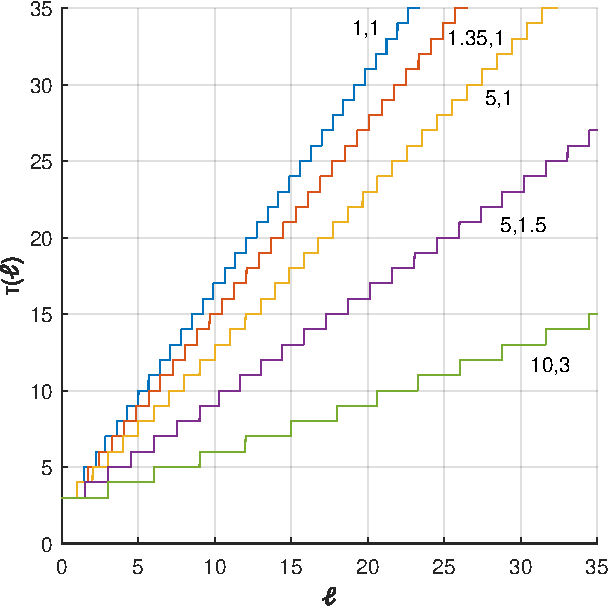
\includegraphics[width=.49\textwidth]{funt_examples}%
}\hfill%
\subfigure[Function $\funl$]{%
\label{fig: funl examples}%
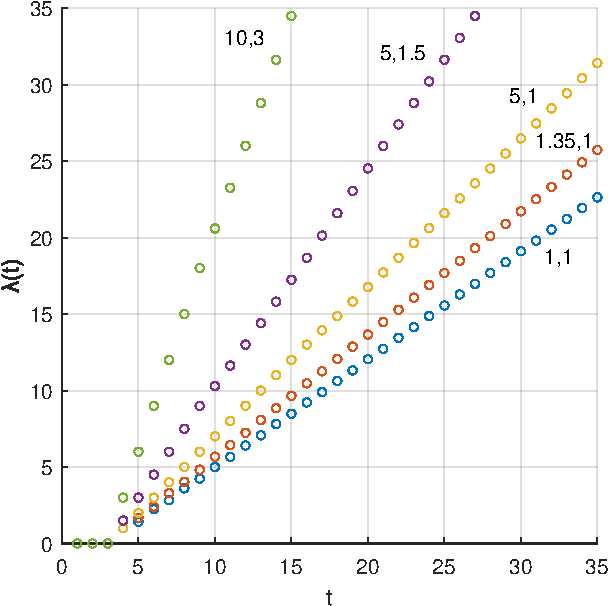
\includegraphics[width=.49\textwidth]{funl_examples}%
}%
\caption{Functions $\funt$ and $\funl$ for several pairs $a$, $b$
}%
\label{fig: funt funl examples}%
\end{figure}%


\subsection{Unit square grid with real-valued lengths}
\label{part: max: unit square grid, real lengths}

A square grid has $a=b$. For real-valued segment lengths it can be further assumed that $a=1$. For $a \neq 1$ the results to be obtained apply with $\len$ replaced by $\len/a$.

Particularizing the results in \S\ref{part: max: arbitrary grid, real lengths} to $a=b=1$ obviously yields simpler formulas.

\begin{corollary}
\label{cor: funt, sq, form}
For a unit square grid with $\len \in \mathbb R^+$,
\begin{equation}
\label{eq: cor: funt, sq, form}
\funt(\len) = \isoli+\jsoli-1
\end{equation}
with
\begin{align}
\label{eq: cor: funt, sq, form; i}
\isoli &= \left\lceil \frac{1 + \Re \sqrt{2\len^2-1}}{2} \right\rceil + 1, \\
\label{eq: cor: funt, sq, form; j}
\jsoli &= \left\lceil \sqrt{\len^2-(\isoli-2)^2} \right\rceil + 1,
\end{align}
\end{corollary}

\begin{corollary}
\label{theo: funl, sq, form}
For a unit square grid, and for $\tiles \in \mathbb N$,
\begin{equation}
\funl(\tiles) = \begin{cases}
\displaystyle
0 & \text{for } \tiles =1, 2 \\[1.4mm]
\displaystyle
\frac{\tiles-3}{\sqrt{2}} & \text{for } \tiles \text{ odd, } \tiles \geq 3 \\[4.5mm]
\displaystyle
\sqrt{\frac{(\tiles-3)^2+1} {2}} & \text{for } \tiles \text{ even, } \tiles \geq 4,
\end{cases}
\end{equation}
or equivalently
\begin{equation}
\label{eq: theo: funt, sq, form; funl}
\funl(\tiles) = \begin{cases}
\displaystyle
0 & \text{for } \tiles =1, 2 \\[1.4mm]
\displaystyle
\sqrt{\left\lceil \frac{(\tiles-3)^2} {2} \right\rceil} & \text{for } \tiles \geq 3.
\end{cases}
\end{equation}
\end{corollary}

Furthermore, an even simpler formula can be obtained for $\funt$, as the next theorem shows.

\begin{theorem}
\label{theo: funt, sq, form}
For a unit square grid with $\len \in \mathbb R^+$,
\begin{equation}
\label{eq: theo: funt, sq, form; funt, with i, j}
\funt(\len) = \isoli+\jsoli-1
\end{equation}
with
\begin{align}
\label{eq: theo: funt, sq, form; i}
\isoli &= \left\lceil \frac{\len}{\sqrt{2}} \right\rceil + 1, \\
\label{eq: theo: funt, sq, form; j}
\jsoli &= \left\lceil \sqrt{\len^2-(\isoli-2)^2} \right\rceil + 1.
\end{align}
Equivalently,
\begin{equation}
\label{eq: theo: funt, sq, form; funt, simpler}
\funt(\len) = \left\lfloor \sqrt{2 \left\lceil \len^2 \right\rceil - 2} \right\rfloor + 3.
\end{equation}
\end{theorem}

\begin{proof}
The proof of \eqref{eq: theo: funt, sq, form; funt, with i, j} uses a variation of the set $\mss$ defined in Proposition~\ref{prop: min suff set, form} that is more suited to this situation.

For $a=b=1$, the set $\mss$ consists of points of the form $(i,i)$ and $(i,i-1)$, as is easily seen from Proposition~\ref{prop: min suff set, form}, and as illustrated in Figure~\ref{fig: pairs_bounds_1}. By symmetry, replacing each point $(i,i-1)$ by $(i-1,i)$ gives a set $\mss'$ which is also optimal. For this new set, the lower bounding line \eqref{eq: lower bound, line} can be replaced by the simpler $j=i$. The same approach used in the proof of Theorem~\ref{theo: funt, form} can be followed, but using this line. Thus $(\isolr, \jsolr)$ is obtained from
\begin{align}
(\isolr-2)^2 + (\jsolr-2)^2  &= \len^2, \\
\jsolr &= \isoli,
\end{align}
which gives
\begin{equation}
\label{eq: theo: funt, sq, form; proof 1}
\isolr = \len/\sqrt{2} + 2.
\end{equation}
The pair $(\isoli,\jsoli)$ resulting from \eqref{eq: theo: funt, sq, form; proof 1} is in $\mss'$, and is given in \eqref{eq: theo: funt, sq, form; i} and \eqref{eq: theo: funt, sq, form; j}. This establishes \eqref{eq: theo: funt, sq, form; funt, with i, j}.

To show \eqref{eq: theo: funt, sq, form; funt, simpler}, it is first noted that for $\tiles \geq 3$ Corollary~\ref{theo: funl, sq, form} gives
\begin{equation}
\funl(\tiles) = \sqrt{\left\lceil \frac{(\tiles-3)^2} {2} \right\rceil}.
\end{equation}
According to \eqref{eq: funt funl}, the function $\funt(\len)$ is given by the largest positive integer $t$ such that 
\begin{equation}
\label{eq: theo: funt, sq, form; proof 2}
\left\lceil \frac{(\tiles-3)^2} {2} \right\rceil < \len ^ 2.
\end{equation}
Since the left-hand side of \eqref{eq: theo: funt, sq, form; proof 2} is an integer, the condition of being strictly less than $\len^2$ is equivalent to
\begin{equation}
\left\lceil \frac{(\tiles-3)^2} {2} \right\rceil  \leq \left\lceil \len^2 \right\rceil  - 1,
\end{equation}
which in turn is the same as
\begin{equation}
\frac{(\tiles-3)^2} {2}\leq  \left\lceil \len^2 \right\rceil  - 1. 
\end{equation}
Finally, solving for $\tiles$ gives
\begin{equation}
\label{eq: theo: funt, sq, form; proof 3}
\tiles \leq \sqrt{2 \left\lceil \len^2 \right\rceil -2 } + 3.
\end{equation}
The desired quantity $\funt(\len)$, that is the largest positive integer $\tiles$ satisfying \eqref{eq: theo: funt, sq, form; proof 3}, is thus the right-hand side rounded down, as given by \eqref{eq: theo: funt, sq, form; funt, simpler}.
\end{proof}

From Theorem~\ref{theo: funt, sq, form} it is easily seen that odd values of $\funt(\len)$ correspond to $\isoli = \jsoli$, whereas even values are achieved with $\jsoli = \isoli+1$. Given $\tiles \geq 3$ with $\tiles$ odd, $\funt(\len) = \tiles$ if and only
\begin{equation}
\label{eq: square, odd max tiles, lengths}
\len \in \left( \frac{\tiles-3}{\sqrt{2}}, \frac{ \sqrt{(\tiles-1)^2+(\tiles-3)^2}}{2} \right].
\end{equation}
For $\tiles \geq 4$, $\tiles$ even, $\funt(\len) = \tiles$ if and only if
\begin{equation}
\label{eq: square, even max tiles, lengths}
\len \in \left(\frac{ \sqrt{(\tiles-2)^2+(\tiles-4)^2}}{2}, \frac{\tiles-2}{\sqrt{2}} \right].
\end{equation}


\subsection{Unit square grid with integer lengths}
\label{part: max: unit square grid, integer lengths}

A natural variation of the first two problems introduced in \S\ref{part: intro} is to consider $a=b=1$ with the additional restriction that the segment length can only be a positive integer (equivalently, the square grid has spacing $a$ and the segment length can only be an integer multiple of $a$).

The \emph{direct problem} in this setting corresponds to the restriction of the function $\funt$ to $\mathbb N$. This will be denoted as a function $\funti: \mathbb N \to \mathbb N$ for greater clarity, although obviously $\funti(\leni) = \funt(\leni)$ for all $\leni \in \mathbb N$. The sequence $\funti(\leni)$, $\leni \in \mathbb N$, which takes values $3, 5, 7, 8, 9, \ldots$, is depicted in Figure~\ref{fig: funti}. This is A346232 in the On-Line Encyclopedia of Integer Sequences \cite{OEIS_unitsq_int_dir}. For this sequence, the expression in Theorem~\ref{theo: funt, sq, form} simplifies in the obvious way, and the following properties hold.

\begin{figure}%
\centering%
\subfigure[Sequence $\funti$]{%
\label{fig: funti}%
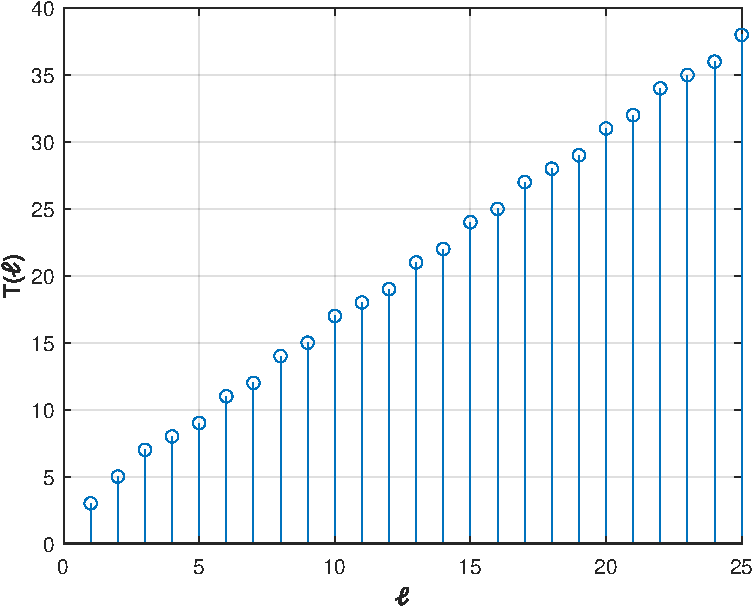
\includegraphics[width=.49\textwidth]{funti}%
}\hfill%
\subfigure[Sequence $\funli$]{%
\label{fig: funli}%
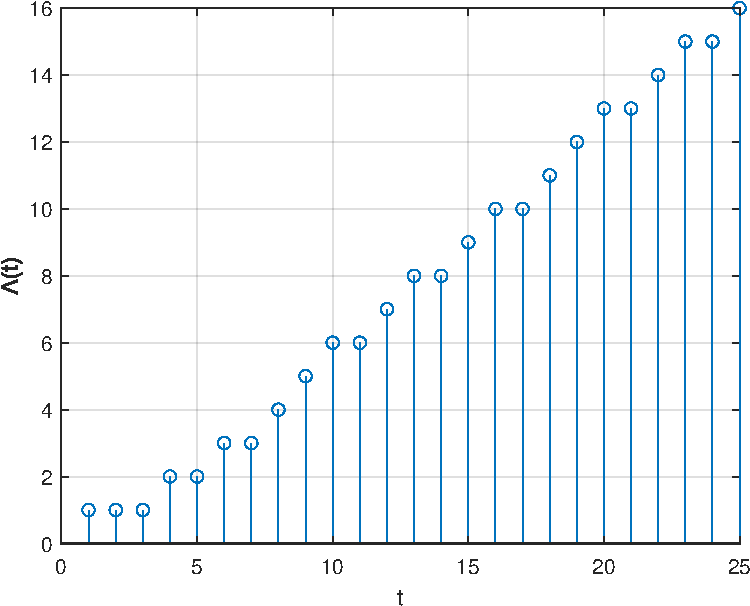
\includegraphics[width=.49\textwidth]{funli}%
}%
\caption{Sequences $\funti$ and $\funli$
}%
\label{fig: funti funti}%
\end{figure}%

\begin{theorem}
\label{theo: funti}
For $\leni \in \mathbb N$,
% $\funti(\leni)$ can be computed as
\begin{equation}
\label{eq: funti leni}
\funti(\leni) = \left\lfloor \sqrt{2\leni^2-2} \right\rfloor + 3.
\end{equation}
In addition,
\begin{enumerate}
\item
This sequence is increasing, with $\funti(\leni+1)-\funti(\leni) \in \{1, 2\}$.
\item
There can be no more than $2$ consecutive increments equal to $1$.
\item
Increments equal to $2$ always appear isolated, except at the initial sequence terms $3, 5, 7$.
\end{enumerate}
\end{theorem}

\begin{proof}
The equality \eqref{eq: funti leni} stems from \eqref{eq: theo: funt, sq, form; funt, simpler} noting that $\len$ is an integer.

In order to prove that $\funti(\leni+1)-\funti(\leni) \in \{1,2\}$, consider the function $\genfun(\genvar) = \sqrt{2\genvar^2-2}$ for $\genvar \in \mathbb R$, $\genvar>1$. Its first derivative is
\begin{equation}
\genfun'(\genvar) = \frac {\sqrt{2} \, \genvar} {\sqrt{\genvar^2-1}},
\end{equation}
and its second derivative is easily seen to be negative. Therefore $\genfun'(\genvar)$ can be bounded for $\genvar \geq 3$ as
\begin{equation}
\label{eq: der bounds}
\lim_{\genvar \rightarrow \infty} \genfun'(\genvar) = \sqrt{2} < \genfun'(\genvar) < \genfun'(3) = 3/2.
\end{equation}
For $\leni \geq 2$, by the mean value theorem \cite[section~5.3]{Abbott15}, when $\leni$ is increased to $\leni+1$ the term $\sqrt{2\leni^2-2}$ in \eqref{eq: funti leni} has an increment that equals $\genfun'(\genvar)$ for some $\leni < \genvar < \leni+1$. Therefore
\begin{equation}
\label{eq: der bounds 2}
\sqrt{2} < \sqrt{2(\leni+1)^2-2} - \sqrt{2\leni^2-2} < 3/2.
\end{equation}
Since $1 < \sqrt{2}$ and $3/2 < 2$, \eqref{eq: der bounds 2} implies that $\funti(\leni+1)-\funti(\leni)$ can only take the values $1$ or $2$ for $\leni \geq 3$. In addition, $\funti(2)-\funti(1) = \funti(3)-\funti(2) = 2$, and thus the result holds for all $\leni \in \mathbb N$.

Using the first bound in \eqref{eq: der bounds 2} three times,
\begin{equation}
3\sqrt{2} < \sqrt{2(\leni+3)^2-2} - \sqrt{2\leni^2-2}.
\end{equation}
Considering that $4 < 3\sqrt{2}$, this implies that $\funti(\leni+3)-\funti(\leni) \geq 4$ for $\leni \geq 3$. Therefore at least one of the three increments from $\funti(\leni)$ to $\funti(\leni+3)$ is $2$. Since $\funti(2)-\funti(1) = \funti(3)-\funti(2) = 2$, the result holds for all $\leni \in \mathbb N$.

Similarly, using the second bound in \eqref{eq: der bounds 2} twice,
\begin{equation}
\sqrt{2(\leni+2)^2-2} - \sqrt{2\leni^2-2} < 3,
\end{equation}
which implies that $\funti(\leni+2)-\funti(\leni) \leq 3$ for $\leni \geq 3$. Therefore the two increments $\funti(\leni+1)-\funti(\leni)$ and $\funti(\leni+2)-\funti(\leni+1)$ cannot both be $2$ for $\leni \geq 3$.
\end{proof}

The \emph{inverse problem} with integer-length segments can be formulated as follows: given $\tiles \in \mathbb N$, find the \emph{minimum} integer length that allows visiting at least $\tiles$ tiles. Observe that in this case, unlike with real-valued lengths, there is indeed a minimum length, because every subset of $\mathbb N$ has a minimum. This can be expressed as a function $\funli: \mathbb N \to \mathbb N$:
\begin{equation}
\label{eq: funli funti}
\funli(\tiles) = \min\{\leni \in \mathbb N \st \funti(\leni) \geq \tiles\},
\end{equation}
which is related to the function $\funl$ corresponding to real-valued lengths by
\begin{equation}
\label{eq: funli funl}
\funli(\tiles) = \lfloor\funl(\tiles)\rfloor + 1.
\end{equation}
The converse to \eqref{eq: funli funti} is (compare to \eqref{eq: funt funl}):
\begin{equation}
\label{eq: funti funli}
\funti(\leni) = \max \{\tiles \in \mathbb N \st \funli(\tiles) \leq \leni\}.
\end{equation}
In view of \eqref{eq: funli funti} and \eqref{eq: funti funli}, $\funti$ and $\funli$ can be considered as ``pseudo-inverse'' sequences of each other.

The sequence $\funli(\tiles)$, $\tiles \in \mathbb N$ can be computed using \eqref{eq: theo: funt, sq, form; funl} and \eqref{eq: funli funl}, and has initial values $1, 1, 1, 2, 2, 3, 3, 4, 5 \ldots$, as shown in Figure~\ref{fig: funli}. This is A346693 in the On-Line Encyclopedia of Integer Sequences \cite{OEIS_unitsq_int_inv}. However, a slightly simpler expression can be obtained from \eqref{eq: funti leni} and \eqref{eq: funli funti}. This is established by the next theorem, which also states some properties of $\funli$, parallel to those of $\funti$.

\begin{theorem}
\label{theo: funli}
For $\tiles \in \mathbb N$,
% $\funli(\tiles)$ can be computed as
\begin{equation}
\label{eq: funli}
\funli(\tiles) = \begin{cases}
\displaystyle
1 & \text{for } \tiles \leq 3 \\[1.3mm]
\displaystyle
\left \lceil \sqrt{\frac{(\tiles-3)^2} 2 + 1} \ \right \rceil & \text{for } \tiles \geq 4.
\end{cases}
\end{equation}
In addition,
\begin{enumerate}
\item
This sequence is non-decreasing. Except for the initial run of $3$ equal values, it is formed by runs of $1$ or $2$ equal values, with an increment of $1$ between consecutive runs.
\item
There can be no more than $3$ different consecutive terms.
\item
A run of $2$ equal values always has $2$ different terms before and $2$ different terms after the run, except for the initial terms $1, 1, 1, 2, 2, 3, 3$.
\end{enumerate}
\end{theorem}

\begin{proof}
Using \eqref{eq: funti leni}, the inequality $\funti(\leni) \geq \tiles$ in \eqref{eq: funli funti} is written as
\begin{equation}
\left\lfloor \sqrt{2\leni^2-2} \right\rfloor + 3 \geq \tiles.
\end{equation}
Since the right-hand side is an integer, this is equivalent to
\begin{equation}
\label{eq: theo funli ineq}
\sqrt{2\leni^2-2} \geq \tiles-3.
\end{equation}
For $\tiles \geq 4$, taking squares and rearranging gives
\begin{equation}
\leni \geq \left \lceil \sqrt{\frac{(\tiles-3)^2} 2 + 1} \ \right \rceil,
\end{equation}
which combined with \eqref{eq: funli funti} yields the second part of \eqref{eq: funli}. The first part results from noting that $\tiles-3 \leq 0$ for $\tiles \leq 3$, and thus $\leni=1$ satisfies \eqref{eq: theo funli ineq}.

The stated properties for $\funli$ follow directly from those of $\funti$ established by Theorem~\ref{theo: funti}.
\end{proof}


\section{Probabilistic characterization for a random segment}
\label{part: rand}

Given $\len \in \mathbb R^+$, consider a segment of length $\len$ with uniformly random position and orientation. Specifically, the coordinates $x_1$, $y_1$ of the first endpoint are independent random variables uniformly distributed on $[0,a)$ and $[0,b)$ respectively. The orientation $\theta$ of the segment is uniformly distributed on $[0,2\pi)$. The variables $x_1$, $y_1$ and $\theta$ determine the coordinates $x_2$, $y_2$ of the second endpoint.

Each realization of the random segment gives rise to a discrete bounding rectangle, whose normalized dimensions $i$ and $j$ are thus random variables, as is the number $\tiles$ of visited tiles. Except for a set of realizations with zero probability, $i$ and $j$ are at least $1$, and $\tiles = i+j-1$ tiles. Note that $i$ and $j$ are not statistically independent. 


\subsection{Arbitrary grid with real-valued lengths}
\label{part: probmax: arbitrary grid, real lengths}

Let $\funta: \mathbb R^+ \to \mathbb R^+$ be defined such that $\funta(\len)$ gives the average number of tiles visited by a random segment of length $\len$, with the distributions specified in \S\ref{part: rand}. This function can be easily computed using the fact that
\begin{equation}
\label{eq: funta E[i] E[j]}
\funta(\len) = \E[\tiles] = \E[i]+\E[j]-1,
\end{equation}
and noting that events of probability $0$, such as $x_1=a$ or the segment passing through a grid point, can be disregarded.

\begin{theorem}
\label{theo: funta, form}
Given $a, b, \len \in \mathbb R^+$, consider a grid with parameters $a, b$ and a uniformly random segment of length $\len$, as defined above. The average number of tiles visited by the segment, $\funta(\len)$, is 
\begin{equation}
\label{eq: funta, form}
\funta(\len) = \frac{2\len}{\pi}\left(\frac 1 a + \frac 1 b\right) + 1.
\end{equation}
\end{theorem}

\begin{proof}
Suppose first that the grid is simplified to only horizontal lines with spacing $b$. This matches the setup of Buffon's original needle problem \cite{Mathai99}, except that here the length $\len$ of the needle may exceed the spacing $b$, allowing it to cross multiple lines. As shown in \cite{Ramaley69}, the expected number of lines crossed equals $2\len/(\pi b)$.
% When $\len<b$ this expectation matches the probability of the needle crossing a grid line, since it cannot cross more than one.

Consider again a grid with horizontal spacing $a$ and vertical spacing $b$. The grid crossings decompose into crossings of horizontal and vertical grid lines. By linearity of expectation, the expected number of crossings $\funca(\len)$ is the sum of the expectations for parallel lines with spacing $a$ and $b$ respectively, which gives
\begin{equation}
\label{eq: funca}
\funca(\len) = \frac{2\len}{\pi}\left(\frac 1 a + \frac 1 b\right).
\end{equation}
As noted in Proposition \ref{prop: i+j-1}, the number of tiles visited by a segment is the count of its grid line crossings plus $1$, unless it exactly passes through any grid points, but that occurs with probability $0$ and therefore does not affect the expectation. Thus, $\funta(\len)$ is given by the right-hand side of \eqref{eq: funca} plus $1$.
\end{proof}

In view of Theorem~\ref{theo: funta, form}, the average number of visited tiles as a function of the segment length has a very simple form, namely an affine function. Conversely, for any $\tiles>1$ it is immediate to compute the length of a random segment that visits $\tiles$ tiles on average, given as $\funta^{-1}(\tiles)$.

In spite of the dependence between the random variables $i$ and $j$, their marginal distributions have relatively simple analytic expressions, as established by the next proposition.

For $0 \leq \genvar \leq 1$, let
\begin{equation}
\label{eq: f}
f(\genvar) = \int_0^\genvar \arccos z \diff z = \genvar \arccos \genvar - \sqrt{1-\genvar^2} + 1.
\end{equation}

\begin{proposition}
\label{prop: Pr i}
Given $a, b, \len \in \mathbb R^+$, consider a grid with parameters $a, b$ and a uniformly random segment of length $\len$, as defined above. Let the random variables $i$, $j$ represent the normalized dimensions of the discrete bounding rectangle. For $n \in \mathbb N$,
\begin{equation}
\label{eq: Pr i geq n}
\Pr[i \geq n] = \begin{cases}
\displaystyle
1 &\text{if\ \ } \displaystyle n =1 \\[1 mm]
\displaystyle
\frac{2\len}{\pi a} \left(f\left(\frac{a(n-1)}{\len}\right)-f\left(\frac{a(n-2)}{\len} \right)\right) &\text{if\ \ } \displaystyle 2 \leq n < \frac \len a + 1 \\[4 mm]
\displaystyle
\frac{2\len}{\pi a}\,\, \left(1 - f\left(\frac{a(n-2)}{\len}\right)\right) &\text{if\ \ } \displaystyle \frac\len a + 1 \leq n < \frac\len a+2 \\[3 mm]
\displaystyle
0 &\text{if\ \ } \displaystyle \frac \len a + 2 \leq  n; \\
\end{cases}
\end{equation}
and $\Pr[j \geq n]$ is given by the same expressions with $a$ replaced by $b$.
\end{proposition}

\begin{proof}
Clearly, $\Pr[i \geq 1]=1$. In the following it will be assumed that $n \geq 2$. The basic idea is to compute $\Pr[i \geq n]$ conditioned on $(x_1,y_1)$ (or, as will be seen, only on $x_1$), and then to average over $x_1$ and $y_1$ (actually only over $x_1$).

Given the coordinates $(x_1, y_1)$ of the first endpoint of the segment, with $0 \leq x_1 \leq a$, $0 \leq y_1 \leq b$, the second endpoint $(x_2, y_2)$ lies on a circle with radius $\len$ centered at $(x_1,y_1)$, as shown in Figure~\ref{fig: Pr_i}. The segment orientation is a random angle $\theta$ uniformly distributed on $[0,2\pi)$. It is clear from the figure that $i \geq n$ if and only if $x_2 \geq a(n-1)$ or $x_2 \leq -a(n-2)$; and these events are exclusive for $n \geq 2$. Thus
\begin{equation}
\label{eq: Pr i cond}
\Pr[i \geq n \cond x_1, y_1] = \Pr[x_2 \geq a(n-1) \cond x_1, y_1] + \Pr[x_2 \leq -a(n-2) \cond x_1, y_1].
\end{equation}
The two conditional probabilities on the right-hand side of \eqref{eq: Pr i cond} are different in general. However, averaging over $x_1, y_1$ gives, by symmetry, $\Pr[x_2 \geq a(n-1)] = \Pr[x_2 \leq -a(n-2)]$. In addition, the coordinate $y_1$ does not have any influence on these events, and therefore conditioning on $x_1, y_1$ is the same as conditioning on $x_1$. This implies that, for $n \geq 2$,
\begin{equation}
\label{eq: Pr i = 2 Pr}
\Pr[i \geq n] = 2 \Pr[x_2 \geq a(n-1)] = 2 \E[\Pr[x_2 \geq a(n-1) \cond x_1]].
\end{equation}

\begin{figure}
\centering%
\subfigure[$x_2$ can exceed $a(n-1)$ for all $x_1$, $0 \leq x_1 \leq a$]{%
\label{fig: Pr_i_full}%
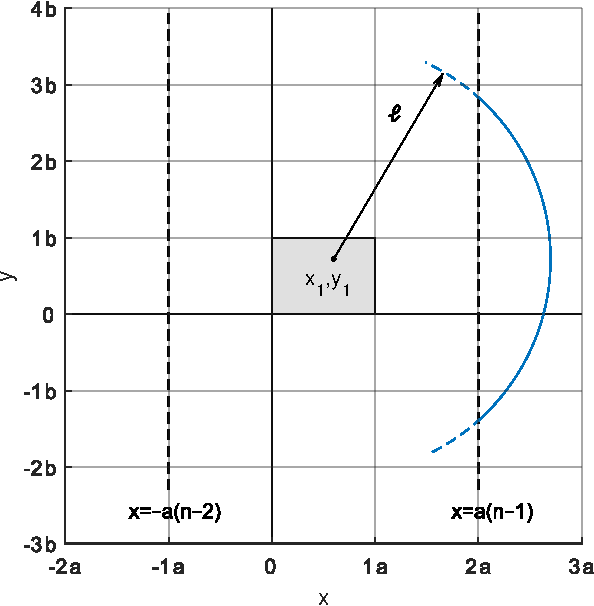
\includegraphics[width=.58\textwidth]{Pr_i_full_1p35}%
}\\%\hfill%
\subfigure[$x_2$ can exceed $a(n-1)$ only if $a(n-1)-\len \leq x_1 \leq a$]{%
\label{fig: Pr_i_notfull}%
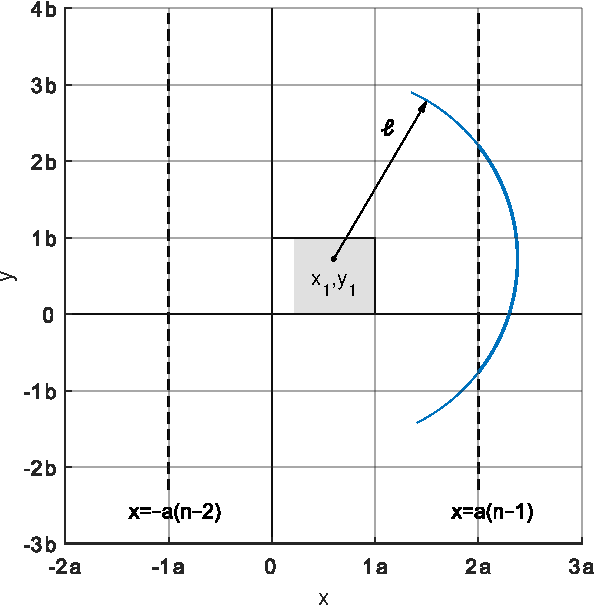
\includegraphics[width=.58\textwidth]{Pr_i_notfull_1p35}%
}%
\caption{Conditions for the normalized width of the discrete bounding rectangle, $i$, to be equal or greater than a given $n$. Example with $a=1.35$, $b=1$, $n=3$
}%
\label{fig: Pr_i}
\end{figure}%

Consider the event $x_2 \geq a(n-1)$ conditioned on $x_1$, with $n \geq 2$. There are three possibilities depending on $x_1$, $n$ and $\len$. If $a(n-1) < \len$, regardless of $x_1$ the length $\len$ is enough for $x_2$ to exceed $a(n-1)$ for some angles $\theta$. This is depicted in Figure~\ref{fig: Pr_i_full}, where the section of the arc with solid line represents those angles for which $x_2 > a(n-1)$. If $a(n-2) < \len \leq  a(n-1)$, the length will be enough provided that $x_1 \geq a(n-1)-\len$, which corresponds to the shaded region in Figure~\ref{fig: Pr_i_notfull}. Lastly, if $\len \leq  a(n-2)$ it is not possible for $x_2$ to exceed $a(n-1)$. Note that the coordinate $y_1$ is irrelevant to this.

In the first two cases above, the probability that $x_2 \geq a(n-1)$, conditioned on $x_1$, is the length of the arc to the right of the line $x=a(n-1)$ divided by $2\pi\len$, that is,
\begin{equation}
\label{eq: Pr x_2 geq a(n-1) cond}
\Pr[x_2 \geq a(n-1) \cond x_1] = \frac 1 \pi \arccos \frac{a(n-1)-x_1}{\len}.
\end{equation}
In the first case $x_1$ has a uniform distribution on $(0,a)$, and $\Pr[x_2 \geq a(n-1)]$ is easily obtained from \eqref{eq: Pr x_2 geq a(n-1) cond} as
\begin{equation}
\label{eq: Pr x_2 geq a(n-1), first case}
\begin{split}
\Pr[x_2 \geq a(n-1)] &= \frac 1 {\pi a} \int_0^a\arccos \frac{a(n-1)-x_1}{\len} \diff x_1 \\
&= \frac{\len}{\pi a}\,\, \left( f\left( \frac{a(n-1)}{\len} \right) - f\left( \frac{a(n-2)}{\len} \right) \right),
\end{split}
\end{equation}
where the function $f$ is defined in \eqref{eq: f}. Substituting into \eqref{eq: Pr i = 2 Pr} yields the result in \eqref{eq: Pr i geq n}, second line.

The second case is similar, but the integration over $x_1$ is from $a(n-1)-\len$ to $a$. Noting that $f(1)=1$, this gives
\begin{equation}
\label{eq: Pr x_2 geq a(n-1), second case}
\Pr[x_2 \geq a(n-1)] = \frac{\len}{\pi a}\,\, \left( 1 - f\left( \frac{a(n-2)}{\len} \right) \right),
\end{equation}
which combined with \eqref{eq: Pr i = 2 Pr} yields the expression in \eqref{eq: Pr i geq n}, third line.

The third case obviously gives $\Pr[i \geq n] = 0$, as in \eqref{eq: Pr i geq n}, fourth line.

The above arguments can be applied to $\Pr[j \geq n]$ if the $x$ and $y$ axes are interchanged. Thus the result is the same with $a$ replaced by $b$.
\end{proof}

The results in Theorem~\ref{theo: funta, form} and Proposition~\ref{prop: Pr i} make clear the relationship between the problem considered in this section here and Buffon's needle problem, i.e.~the probability that a random segment of fixed length crosses a line in a regular structure of parallel strips \cite[section 1.1]{Mathai99}. Firstly, since the number $\pi$ is involved in \eqref{eq: funta, form}, it is possible to design a simple probabilistic experiment to estimate the value of $\pi$, as in Buffon's original experiment. For example, choosing $a=b=\len=1$ gives $\funta(\len) = 1+1/\pi$.

Secondly, a grid with $b \rightarrow \infty$ corresponds to Buffon's arrangement of parallel strips with spacing $a$. Thus
\begin{equation}
\label{eq: number of lines crossed, Buffon}
\lim_{b \rightarrow \infty} \funta(\len)-1 = \frac{2\len}{\pi a}
\end{equation}
gives the average number of lines crossed in Buffon's experiment. For $\len \leq a$ the segment can cross at most one line, and \eqref{eq: number of lines crossed, Buffon} coincides with the probability of crossing \cite[section 1.1]{Mathai99}.

Lastly, $\Pr[i \geq n]$ as computed in Proposition~\ref{prop: Pr i} for $n \geq 2$ can be seen as a generalization of the probability of crossing at least one line in Buffon's experiment, when a needle endpoint is only allowed to move in a narrower region of width $n-1$ times smaller than the width of the strips (instead of across the full strip as in Buffon's setting).

For $\len \rightarrow \infty$, the average number of visited tiles $\funta$ has the following asymptotic slope, as stems from \eqref{eq: funta, form}:
\begin{equation}
\label{eq: asympt slope ave}
\lim_{\len \rightarrow \infty} \frac{\funta(\len)}{\len} = \frac 2 \pi \left(\frac 1 a + \frac 1 b \right).
\end{equation}
On the other hand, the maximum number of visited tiles $\funt$ has an asymptotic slope given by \eqref{eq: asympt slope}. It is interesting to consider the ratio of these values, which also gives the asymptotic ratio of average and maximum numbers of visited tiles. This depends only on $a/b$:
\begin{equation}
\label{eq: ras}
\ras(a/b) = \lim_{\len \rightarrow \infty}
\frac { \funta(\len) } { \funt(\len) }
= \frac
{ \lim_{\len \rightarrow \infty} \funta(\len)/\len }
{ \lim_{\len \rightarrow \infty} \funt(\len)/\len }
= \frac{2\left(1 + a/b\right)}{\pi\sqrt{1 + \left(a/b\right)^2}}.
\end{equation}
The function $\ras$ satisfies $\ras(x) = \ras(1/x)$, and is therefore symmetric in logarithmic scale, as can be seen in Figure~\ref{fig: ratio asympt slopes}. It is unimodal with maximum value $2\sqrt 2/\pi \approx 0.9003$ for $a/b=1$, and its limit when $a/b$ tends to $0$ or $\infty$ is $2/\pi \approx 0.6366$. This implies that for $\len$ large the average number of tiles $\funta(\len)$ cannot very small compared with the maximum number of tiles $\funt(\len)$. For example, $\funta(\len)$ asymptotically exceeds $0.8\funt(\len)$ for $1/3 \leq a/b \leq 3$.

\begin{figure}
\centering%
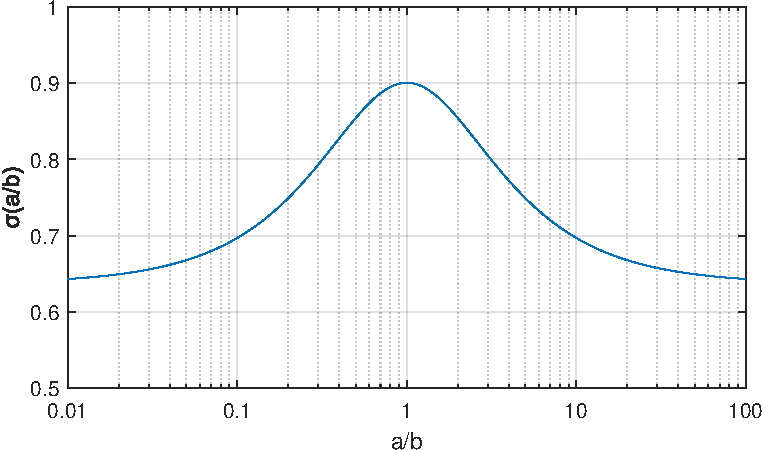
\includegraphics[width=.7\textwidth]{ratio_asympt_slopes}%
\caption{Asymptotic ratio of average and maximum numbers of visited tiles
}%
\label{fig: ratio asympt slopes}%
\end{figure}%

The probability of visiting the maximum number of tiles for a rectangular grid is difficult to compute, due to the irregularity of the optimal $(i,j)$ pairs (see \S\ref{part: fund results}). In the square case, however, the simplicity of the set makes the problem more tractable. 


\subsection{Unit square grid with real-valued lengths}
\label{part: probmax: unit square grid, real lengths}

Consider a square grid with unit spacing, $a=b=1$. Again, the results to follow can be applied to a square grid with spacing $a \neq 1$ if $\len$ is replaced by $\len/a$.

For a random segment with length $\len \in \mathbb R^+$ on a unit square grid, let the function $\probmax: \mathbb R^+ \to [0,1]$ be defined such that $\probmax(\len)$ gives the probability that the segment visits the maximum possible number of tiles, $\funt(\len)$. This function is characterized by the next theorem.

For $u, v \in \mathbb N$, $\genvar \in \mathbb R^+$, let
\begin{equation}
\label{eq: g def}
g(\genvar, u, v) = \int_{\arcsin \frac u {2r}}^{\arccos \frac u {2r}} \left( \genvar \sin \theta - \frac u 2 \right) \left( \genvar \cos \theta - \frac v 2 \right) \diff \theta.
\end{equation}
Using the identities $\cos^2 \alpha = 1-\sin^2 \alpha$ and $\cos(2\alpha) = 2\cos^2\alpha-1 = 1 - 2\sin^2\alpha$, the integral in \eqref{eq: g def} is computed as
\begin{equation}
\label{eq: g fin}
\begin{split}
g(\genvar, u, v) &= \frac 1 {2\pi} \biggl(
\left(\arccos\frac{u}{2\genvar}-\arcsin\frac{v}{2\genvar}\right) u v + 2\genvar^2 + \frac{u^2} 2 + \frac{v^2} 2 \\
& \quad  - u \sqrt{4\genvar^2-v^2} - v \sqrt{4\genvar^2-u^2} \biggr).
\end{split}
\end{equation}

\begin{theorem}
\label{theo: probmax, sq}
Given $\len \in \mathbb R^+$, consider a unit square grid and a uniformly random segment of length $\len$, as previously defined. The probability $\probmax(\len)$ that the segment visits the maximum number of tiles $\funt(\len)$ is
\begin{equation}
\label{eq: probmax}
\begin{split}
\probmax(\len) & = g\left(\len, 
\tiles-3, \tiles-3 \right) \quad\ \text{for } \tiles \text{ odd, } \textstyle \len \in \left( \frac{\tiles-3}{\sqrt{2}}, \frac{\sqrt{(\tiles-5)^2+(\tiles-1)^2}} 2 \right]; \\
\probmax(\len) & = g\left(\len, \tiles-3, \tiles-3 \right) + 2 g\left(\len, \tiles-5, \tiles-1 \right) \\
& \text{for } \tiles \text{ odd, } \textstyle \len \in \left (\frac{\sqrt{(\tiles-5)^2+(\tiles-1)^2}} 2,  \frac{\sqrt{(\tiles-3)^2+(\tiles-1)^2}} 2 \right]; \\
\probmax(\len) & = 2 g\left(\len, \tiles-4, \tiles-2 \right) \quad \text{for } \tiles \text{ even, } \textstyle \len \in \left( \frac{\sqrt{(\tiles-4)^2+(\tiles-2)^2}} 2, \frac{\sqrt{(\tiles-6)^2+\tiles^2}} 2 \right]; \\
\probmax(\len) & = 2 g\left(\len, \tiles-4, \tiles-2 \right) + 2 g\left(\len, \tiles-6, \tiles \right) \\
& \text{for } \tiles \text{ even, } \textstyle \len \in \left( \frac{\sqrt{(\tiles-6)^2+\tiles^2}} 2, \frac{\tiles-2}{\sqrt{2}} \right].
\end{split}
\end{equation}
\end{theorem}

\begin{proof}
The approach is similar to that used in the proof of Proposition~\ref{prop: Pr i}, but conditioning on the segment orientation $\theta$ instead of on the location of its first endpoint.

The first endpoint of the segment is assumed to be in the reference tile with lower-left corner $(0,0)$. For an arbitrary value $\tiles$, the segment visits $\tiles$ tiles almost surely if and only if its second endpoint is in a tile with lower-left corner $(i-1,j-1)$, $i,j\geq 1$, $i+j-1=\tiles$, or in a tile symmetrical to this with respect to the line $x=1/2$ (with $i \leq 0$), or $y=1/2$ (with $j \leq 0$), or both.

Consider $i,j\geq 1$ for the moment, and let $\tiles = \funt(\len)$. For a given orientation $\theta$, the segment goes from the reference tile to that with lower-left corner $(i-1,j-1)$ if and only if shifting the segment so that its second endpoint has coordinates $(i-1,j-1)$ results in the first endpoint being in the reference tile. It cannot be the case that the segment ``overshoots'' past this tile, because that would result in a number of visited tiles exceeding the assumed maximum, $\tiles$.

\begin{figure}
\centering%
\subfigure[The second endpoint is in the tile with lower-left corner $((\tiles-1)/2,(\tiles-1)/2)$]{%
\label{fig: probmax_funt_odd_diag}%
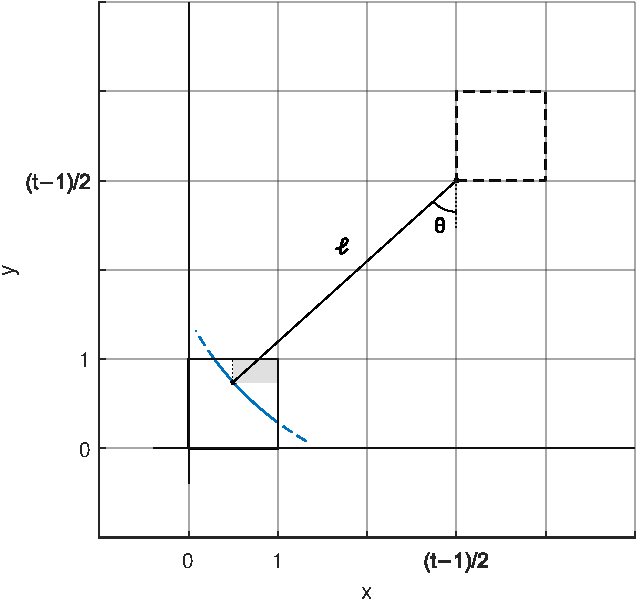
\includegraphics[width=.56\textwidth]{probmax_funt_odd_diag}%
}\\%\hfill%
\subfigure[The second endpoint is in the tile with lower-left corner $((\tiles-3)/2,(\tiles+1)/2)$]{%
\label{fig: probmax_funt_odd_offdiag}%
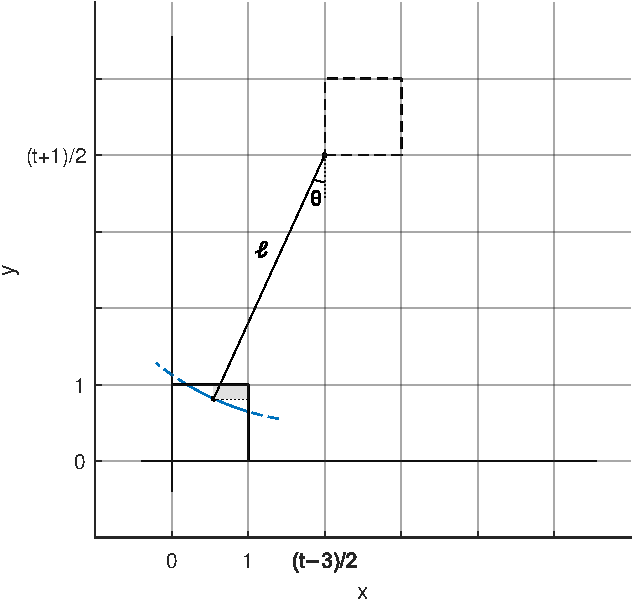
\includegraphics[width=.56\textwidth]{probmax_funt_odd_offdiag}%
}%
\caption{Segment orientations and positions of the first endpoint within the reference tile for a given number $\tiles$ of visited tiles. Example for odd $\tiles$
}%
\label{fig: probmax_funt_odd}%
\end{figure}%

There is a range of possible values of $\theta$ for which the above condition is satisfied. This range corresponds to the part of the arc with solid line in Figure~\ref{fig: probmax_funt_odd}. For convenience, the angle $\theta$ is defined clockwise from the downward direction. For each $\theta$ in the allowed range, the valid positions for the first endpoint of the (shifted) segment are in the shaded rectangle, whose dimensions depend on $\theta$. The area occupied by this rectangle is the probability $\probmax_{i-1,j-1}(\len,\theta)$ that the segment goes from the reference tile to that with lower-left corner $(i-1,j-1)$ conditioned on $\theta$. The desired probability, $\probmax(\len)$, will be obtained by averaging $\probmax_{i-1,j-1}(\len, \theta)$ over $\theta$, summing over all $i, j \geq 1$ such that the tile with lower-left corner $(i-1, j-1)$ can be reached from the reference tile, and then using symmetry to take into account the tiles with $i \leq 0$ or $j \leq 0$.

The situation is different depending on whether $\tiles$ is odd or even. Consider $\tiles$ odd first. Under this assumption, the range of lengths corresponding to the condition $\tiles = \funt(\len)$ is given by \eqref{eq: square, odd max tiles, lengths}. For any length in this interval, there are some positions within the reference tile from which the tile with lower-left coordinate $((\tiles-1)/2, (\tiles-1)/2)$ can be reached. Equivalently, the shifted segment with one endpoint at $((\tiles-1)/2, (\tiles-1)/2)$ can reach the reference tile. This is illustrated in Figure~\ref{fig: probmax_funt_odd_diag}. In addition, if 
\begin{equation}
\label{eq: probmax len odd2}
\len > \frac{\sqrt{(\tiles-5)^2 + (\tiles-1)^2}}{2}
\end{equation}
the two tiles with lower-left coordinates $((\tiles-3)/2, (\tiles+1)/2)$ and $((\tiles+1)/2, (\tiles-3)/2)$ are also reachable from the reference tile; or equivalently the shifted segment can reach the reference tile, as shown in Figure~\ref{fig: probmax_funt_odd_offdiag}. This can only happen for $\tiles \geq 5$ (for $\tiles=3$ the inequality \eqref{eq: probmax len odd2} cannot be satisfied for lengths in the range given by \eqref{eq: square, odd max tiles, lengths}). In this case, by symmetry, each of those two tiles contributes the same probability. Other tiles with $i,j\geq 1$ corresponding to the same $\tiles$ do not need to be considered, because they cannot be reached with lengths satisfying \eqref{eq: square, odd max tiles, lengths}.

For $\tiles$ even, which corresponds to lengths in the interval \eqref{eq: square, even max tiles, lengths}, the two tiles with lower-left coordinates $(\tiles/2-1, \tiles/2)$ and $(\tiles/2, \tiles/2-1)$ can always be reached from some positions within the reference tile. In addition, if
\begin{equation}
\label{eq: probmax len even2}
\len > \frac{\sqrt{((\tiles-6)^2 + \tiles^2}}{2}
\end{equation}
the two tiles with lower-left coordinates $(\tiles/2-2, \tiles/2+1)$ and $(\tiles/2+1, \tiles/2-2)$ have to be considered too. This can only happen for $\tiles \geq 8$. No other tiles with $i,j\geq 1$ can be reached from the reference tile.

The above two paragraphs show that, among all possible tiles with lower-left corner $(i-1,j-1)$, $i,j\geq 1$, those whose centers lie on the lines $x=1/2$ or $y=1/2$ (i.e.~those with $i=1$ of $j=1$) are never reachable from the reference tile, in the sense that a segment that touches the maximum number of tiles cannot have its second endpoint in those tiles. This implies that $\probmax(\len)$ can be computed by considering only the tiles with $i,j\geq 1$ (actually $i,j \geq 2$), and then multiplying by $4$ to include the symmetrical tiles with respect to $x=1/2$ and $y=1/2$. As an example, Figure~\ref{fig: probmax_possible_tiles} shows the reference tile (solid line) and the tiles that can contain the second endpoint (dotted lines) for $\funt(\len) = 5$.

\begin{figure}
\centering%
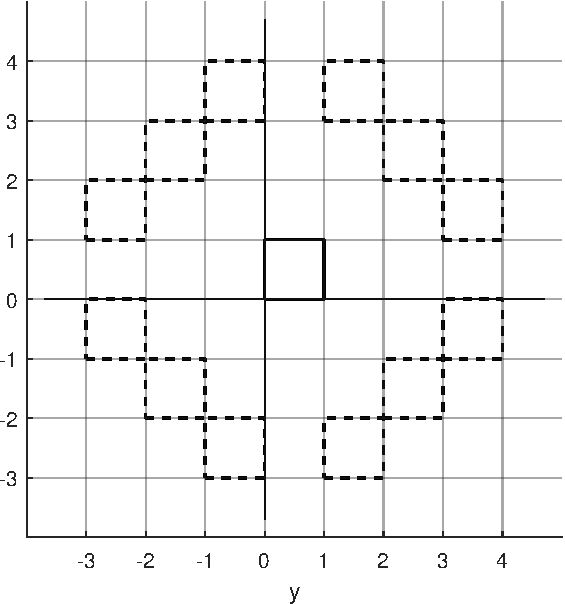
\includegraphics[width=.52\textwidth]{probmax_possible_tiles}%
\caption{Tiles that can contain the second endpoint of a segment that visits the maximum number of tiles $\funt(\len)$ in a square grid (example for $\funt(\len)=5$)%
}%
\label{fig: probmax_possible_tiles}%
\end{figure}%

According to the preceding analysis, two cases need to be distinguished for $\tiles$ odd, depending on whether \eqref{eq: probmax len odd2} is satisfied or not; and similarly two cases exist for $\tiles$ even, depending on whether \eqref{eq: probmax len even2} holds or not. These are, respectively, the four cases in \eqref{eq: probmax}.

In the first case indicated in \eqref{eq: probmax}, as argued, $\tiles$ is odd and only the tile with lower-left coordinates $((\tiles-1)/2, (\tiles-1)/2)$ is reachable. For a given $\theta$, the conditional probability $\probmax_{(\tiles-1)/2, (\tiles-1)/2}(\len, \theta)$ is the area of the shaded rectangle in Figure~\ref{fig: probmax_funt_odd_diag}:
\begin{equation}
\label{eq: probmax: probmax theta odd}
\probmax_{(\tiles-1)/2, (\tiles-1)/2}(\len, \theta) = \left(\len\sin\theta - \frac{\tiles-3}2\right) \left(\len\cos\theta - \frac{\tiles-3}2\right).
\end{equation}
The range of allowed values for $\theta$, as can be seen from the figure, is $(\theta_0, \theta_1)$ with
\begin{align}
\label{eq: odd theta 0}
\theta_0 & = \arcsin\frac{\tiles-3}{2\len}, \\
\label{eq: odd theta 1}
\theta_1 & = \arccos\frac{\tiles-3}{2\len}.
\end{align}
Computing the average of \eqref{eq: probmax: probmax theta odd} over $\theta$, multiplying by $4$ to include all quadrants and comparing with \eqref{eq: g def} gives $\probmax(\len)$ as
\begin{equation}
\label{eq: probmax: probmax odd}
\begin{split}
\probmax(\len) & = 4 \int_{\theta_0}^{\theta_1} \frac{\probmax_{(\tiles-1)/2, (\tiles-1)/2}(\len, \theta)}{2\pi} \diff \theta \\
& = \frac 2 \pi \int_{\arcsin\frac{\tiles-3}{2\len}}^{\arccos\frac{\tiles-3}{2\len}} \left( \len\sin\theta - \frac{\tiles-3} 2 \right)  \left( \len\cos\theta - \frac{\tiles-3} 2 \right) \diff \theta \\
& = g\left( \len, \tiles-3, \tiles-3 \right ),
\end{split}
\end{equation}
in accordance with \eqref{eq: probmax}.

For the second case in \eqref{eq: probmax}, $\probmax(\len)$ is obtained as above plus an additional term corresponding to the tile with lower-left corner $((\tiles-3)/2, (\tiles+1)/2)$, multiplied by $2$ to account for its symmetrical tile about the line $y=x$, namely that with lower-left corner $((\tiles+1)/2, (\tiles-3)/2)$, and by $4$ to include all quadrants. Observing the shaded rectangle in Figure~\ref{fig: probmax_funt_odd_offdiag},
\begin{equation}
\label{eq: probmax: probmax theta odd2}
\probmax_{(\tiles-3)/2, (\tiles+1)/2}(\len, \theta) = \left(\len\sin\theta - \frac{\tiles-5}2\right) \left(\len\cos\theta - \frac{\tiles-1}2\right).
\end{equation}
The integration interval $(\theta_0, \theta_1)$ is in this case
\begin{align}
\theta_0 & = \arcsin\frac{\tiles-5}{2\len}, \\
\theta_1 & = \arccos\frac{\tiles-1}{2\len}.
\end{align}
The additional contribution to $\probmax(\len)$, given by
\begin{multline}
8 \int_{\theta_0}^{\theta_1} \frac{\probmax_{(\tiles-3)/2, (\tiles+1)/2}(\len, \theta)}{2\pi} \diff \theta \\
= \frac 4 \pi \int_{\arcsin\frac{\tiles-5}{2\len}}^{\arccos\frac{\tiles-1}{2\len}} \left( \len\sin\theta - \frac{\tiles-5} 2 \right)  \left( \len\cos\theta - \frac{\tiles-1} 2 \right) \diff \theta,
\end{multline}
is recognized to be $2 g(\len, \tiles-5, \tiles-1)$. This proves the second equality in \eqref{eq: probmax}.

The expressions for the third and fourth cases in \eqref{eq: probmax}, corresponding to $\tiles$ even, are established analogously.
\end{proof}

The technique used in the proof of Theorem~\ref{theo: probmax, sq} could in principle be used for obtaining the probability that the number of tiles visited by the segment equals or exceeds any given value $t < \funt(\len)$. The resulting expressions, however, are cumbersome, because more cases (more subintervals for the length) need to be distinguished depending on how many tiles with lower-left corner $(i-1,j-1)$ such that $i+j-1=t$ can be reached from the reference tile.

\begin{figure}%
\centering%
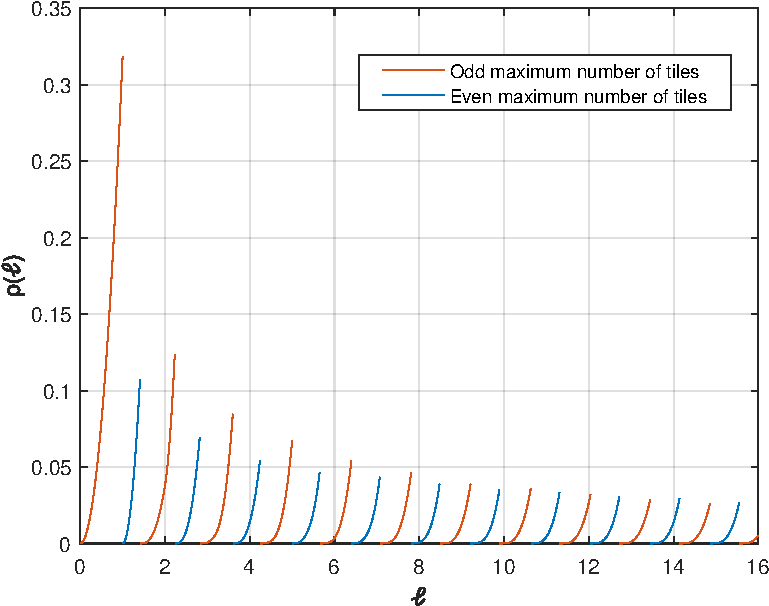
\includegraphics[width=.75\textwidth]{probmax_len}%
\caption{Probability $\probmax(\len)$ that a random segment of length $\len$ visits the maximum number of tiles%
}%
\label{fig: probmax_len}%
\end{figure}%

Figure~\ref{fig: probmax_len} shows the probability $\probmax(\len)$ of visiting the maximum number of tiles on a unit square grid, as given by \eqref{eq: probmax}. As $\len$ grows, $\probmax(\len)$ has a jump when the maximum number of tiles that can be visited increases by $1$ (and there the function takes the value approached from the left). This happens when $\len$ equals the right endpoint of the interval \eqref{eq: square, odd max tiles, lengths} for $\tiles$ odd or of \eqref{eq: square, even max tiles, lengths} for $\tiles$ even. Let these length values be denoted as $\len_\tiles$:
\begin{equation}
\len_\tiles = \begin{cases}
\displaystyle
\frac{\sqrt{(\tiles-3)^2 + (\tiles-1)^2}} {2} & \text{ for $\tiles$ odd, $\tiles \geq 3$} \\
\displaystyle
\frac{\tiles-2}{\sqrt{2}} & \text{ for $\tiles$ odd, $\tiles \geq 4$}.
\end{cases}
\end{equation}
For example, the first continuous section seen in Figure~\ref{fig: probmax_len} corresponds to a maximum number of tiles $\tiles=3$, for lengths in the interval $(0, \len_3]$, where $\len_3= 1$. The second corresponds to $\tiles=4$, for lengths in $(\len_3, \len_4]$, where $\len_4= \sqrt{2}$. Within each continuous section the probability monotonically increases from $0$ to a maximum value. The heights of the maxima follow different trends for odd and even $\tiles$ respectively, as can be seen in the figure; but in each case they are asymptotically proportional to $1/\len_\tiles$. This is established by the next result.

\begin{proposition}
The function $\probmax$ has the following asymptotic behaviour:
\begin{align}
\label{eq: probmax liminf}
\liminf_{\len \rightarrow \infty}\, \probmax(\len) & = 0 \\ 
\label{eq: probmax lim odd}
\lim_{\substack{\tiles \rightarrow \infty \\
\tiles \ \mathrm{odd}}}\, \tiles \probmax(\len_\tiles) & = \frac 2 \pi \\
\label{eq: probmax lim even}
\lim_{\substack{\tiles \rightarrow \infty \\ \tiles \ \mathrm{even}}}\, \tiles \probmax(\len_\tiles) & = \frac 8 {3\pi} \\
\label{eq: probmax limsup}
\limsup_{\len \rightarrow \infty}\, \len \probmax(\len) & = \frac {4\sqrt{2}}{3\pi}.
\end{align}
\end{proposition}

\begin{proof}
The probability $\probmax(\len)$ becomes $0$ whenever the length causes the maximum number of visited tiles to increase by $1$. This establishes \eqref{eq: probmax liminf}.

For \eqref{eq: probmax lim odd} it suffices to note that
\begin{align}
\label{eq: tedious limit, odd 1}
\lim_{\tiles \rightarrow \infty}\, \tiles g\left(\frac{\sqrt{(\tiles-3)^2+(\tiles-1)^2}} 2, \tiles-3, \tiles-3 \right) &= \frac 2 {3\pi} \\
\label{eq: tedious limit, odd 2}
\lim_{\tiles \rightarrow \infty}\, \tiles g\left(\frac{\sqrt{(\tiles-3)^2+(\tiles-1)^2}} 2, \tiles-5, \tiles-1 \right)
& = \frac 2 {3\pi},
\end{align}
as can be (somewhat tediously) checked using L'H\^opital's rule \cite[section~5.3]{Abbott15}.
%***I think. It's very tedious by hand. I used Maple to compute the limit, and then checked it numerically. Maybe one or two intermediate steps from applying L'H\^opital's rule should be included. Perhaps those can be obtained with Maple too, and this part can be rewritten.
Combining these expressions with the second equality in \eqref{eq: probmax} yields \eqref{eq: probmax lim odd}.

Similarly,
\begin{align}
\label{eq: tedious limit, even 1}
\lim_{\tiles \rightarrow \infty}\, \tiles g\left(\frac{\tiles-2}{\sqrt 2}, \tiles-4, \tiles-2 \right) &= \frac 2 {3\pi} \\
\label{eq: tedious limit, even 2}
\lim_{\tiles \rightarrow \infty}\, \tiles g\left(\frac{\tiles-2}{\sqrt 2}, \tiles-6, \tiles \right)
& = \frac 2 {3\pi},
\end{align}
and combining with the fourth equality in \eqref{eq: probmax} gives \eqref{eq: probmax lim even}.

For large $\tiles$, $\len_\tiles$ asymptotically approaches $\tiles/\sqrt{2}$. Using this into \eqref{eq: probmax lim even}, which is greater than \eqref{eq: probmax lim odd}, yields \eqref{eq: probmax limsup}.
\end{proof}


\bibliographystyle{plain}
\bibliography{bibliogr/lista_local}


\end{document}